

\documentclass[12pt]{article}
\usepackage[a4paper, total={6.5in, 9.5in}]{geometry}

\usepackage[en-GB]{datetime2}
\usepackage[parfill]{parskip}
\usepackage{graphicx,caption,fancyhdr,xcolor,pdfpages,setspace}
\usepackage{minted}
\usepackage{amsmath}
\usepackage{amssymb}
\usepackage{titlesec}
\usepackage{CJKutf8}
\usepackage{placeins}
\usepackage{siunitx}


\usepackage[
    colorlinks=true,
	linkcolor=darkgray,
	citecolor=red,
	urlcolor=red
]{hyperref}

\setlength\emergencystretch{2pt}
\titleclass{\subsubsubsection}{straight}[\subsection]

\newcounter{subsubsubsection}[subsubsection]
\numberwithin{subsubsubsection}{subsubsection}

\titleformat{\subsubsubsection}{\normalfont\normalsize\bfseries}{\thesubsubsubsection}{1em}{}
\titlespacing*{\subsubsubsection}{0pt}{3.25ex plus 1ex minus .2ex}{1.5ex plus .2ex}

\makeatletter
\def\toclevel@subsubsubsection{4}
\def\l@subsubsubsection{\@dottedtocline{4}{7em}{4em}}
\makeatother

\setcounter{secnumdepth}{4}
\setcounter{tocdepth}{4}

\usepackage[english]{babel}
\usepackage[square,numbers]{natbib}


\setlength{\fboxsep}{1em}

\urlstyle{same}
\renewcommand{\footnoterule} % Push footnotes to the bottom of the page
	{\vfill\kern -3pt \hrule width 0.4\columnwidth \kern 2.6pt}

\makeatletter
\title{Ten\begin{CJK}{UTF8}{min}(天)\end{CJK}: A Novel Music Sequencer}
\let\Title\@title
\author{Adam Gottesman}
\let\Author\@author
\date{Semester II, 2024}
\let\Date\@date
\makeatother

\fancypagestyle{content}{
    \renewcommand{\headrulewidth}{.4pt}
    \renewcommand{\footrulewidth}{\headrulewidth}
    \setlength{\headheight}{15pt}
    
	\fancyhf{}
	\fancyhead[L]{\Author}
	\fancyhead[R]{\Title}
	\fancyfoot[L]{\Date}
	\fancyfoot[R]{\thepage}
}
\onehalfspacing

\begin{document}

\thispagestyle{empty}
\begin{center}
    \Large
    BEng Project Final Report
    \par ELE00080H
    \vfill
    \makeatletter
    Ten\begin{CJK}{UTF8}{min}(天)\end{CJK}: A Novel Music Sequencer Inspired by Recurring Decimals and the Complex Plane
    \vfill
    \@author
    \makeatother
    \par\DTMdisplaydate{2024}{5}{20}{Tuesday}
    \vfill
    \textit{University of York}
\end{center}
\clearpage

\titleformat{\chapter}[display]
    {\flushright}
    {\fontsize{96}{96}\selectfont\largetitlestyle\thechapter}
    {0pt}
    {\Huge\titlestyle}
\titlespacing*{\chapter}{0pt}{0pt}{2\baselineskip}

%\pagestyle{content}
\pagenumbering{roman}
\phantomsection
\section*{Abstract}

This document outlines the development of the Complex Plane, a key feature of the innovative music sequencer Ten\begin{CJK}{UTF8}{min}(天)\end{CJK}, designed to generate novel compositions and enhance live performances. By integrating 64 potentiometers and RGB addressable LEDs with an ARM\textsuperscript{\textregistered} STM32F407VG microcontroller, the Complex Plane enables real-time sensor readings and visual feedback. Multichannel sensors are managed through a nine 8:1 Multiplexer setup, with custom algorithms handling node transitions and Serial Peripheral Interface (SPI) communication for efficient LED control. Implemented in bare-metal embedded C using the Common Microcontroller Software Interface Standard (CMSIS) library, the system leverages Direct Memory Access (DMA) functionality to increase operational efficiency. Additionally, a memory optimisation strategy is employed for the SPI communication with RGB addressable LEDs, significantly reducing the system's memory footprint. The wiring design balances a software-centric approach for sequence management with a hardware-centric layout for optimal printed circuit board (PCB) design. Ergonomic considerations lead to the implementation of three-way switches for mode selection, enhancing user experience by reducing cognitive load during operation. Integration with third-party synthesisers is achieved for both control voltage/gate (CV/gate) and MIDI, ensuring broad compatibility. User feedback, gathered through surveys, indicates high usability and innovation, with suggestions for further enhancements. The project adheres to ethical standards, including environmental sustainability and data privacy. 



\newpage

\tableofcontents
\newpage


\newpage

\phantomsection
\section*{Acknowledgements}
\addcontentsline{toc}{section}{Acknowledgements}
I would like to thank my supervisors, Dr. Dave Pearce and Dr. Manish Chauhan, for guiding me throughout the entire project. Dr. Pearce, in particular, responded to countless queries I had, proposed many of the methods I employed, and helped me improve my technical writing skills.

\newpage


\phantomsection
\section*{Statement of Ethics}
\addcontentsline{toc}{section}{Statement of Ethics}
The development of a new music sequencer should address the following: compliance with copyright and patent laws, environmental sustainability and data privacy.

Addressing copyright and patent issues involves transparency in documenting research methods and acknowledging intellectual property.

In terms of environmental sustainability, the selection of the Arm\textsuperscript{\textregistered} STM32F407VG microcontroller (MCU) is significant. This choice is influenced by the supplier's commitment to environmental sustainability \cite{STM3}, aligning the project with global ethical standards.

User surveys will be conducted during the product's development to assess technical benchmarks. Participants will be informed about how their data will be analysed and will provide consent, ensuring transparency and trust. Participation in these surveys is voluntary, and participants have the right to opt out at any time. Managing personal data in compliance with the University of York's adherence to the General Data Protection Regulation and the Data Protection Act \cite{Data1} is crucial. Procedures for data access and security against unauthorised access will be strictly followed.


\newpage





\newpage
\pagenumbering{arabic}
\section{Introduction}
Music sequencers are vital in electronic music production and performance. They enable a level of precision in timing and pitch beyond manual methods. This project aims to open up new entrepreneurial opportunities by offering unique features and responding to the latest trends in music technology.

Research outlined in the \hyperref[appendix:background]{Background} section of the appendix suggests that an innovative music sequencer should communicate effectively with a broad range of third-party synthesisers; feature an intuitive interface to enhance functionality; and employ novel methods for generating and representing rhythmic sequences. To meet these objectives, the sequencer design should integrate sensors and indicators for precise parameter control and visual feedback; incorporate control-voltage/gate (CV/gate) and MIDI functionality for broad compatibility; pursue cost-effective solutions to enhance market competitiveness; and focus on ergonomic and intuitive user interfaces to maximise creative output. Additionally, the project should commit to selecting components that adhere to environmental sustainability.

This document details the development and technical specifications of the Complex Plane, a key component of the Ten\begin{CJK}{UTF8}{min}(天)\end{CJK} music sequencer. It begins with an overview of sensor integration, focusing on real-time data acquisition from 64 potentiometers and comparing the effectiveness of Multiplexer (MUX) and Summing Amplifier topologies for accurate sensor readings. The discussion then shifts to indicator management, particularly the programming of 64 RGB addressable LEDs via Serial Peripheral Interface (SPI) communication protocols, and includes an exploration of a memory optimisation strategy essential for efficient visual feedback. Additionally, the narrative addresses wiring strategies within the Complex Plane, contrasting software-centric and hardware-centric approaches and their implications for printed circuit board (PCB) design. Ergonomic considerations follow, with an evaluation of user interface choices such as switches and buttons designed to enhance usability and reduce cognitive load.

The document further describes the output functionalities of the sequencer, including CV/gate and MIDI integration, detailing how these technologies interface with external synthesisers. User feedback is analysed to assess the usability and innovative aspects of the sequencer, highlighting areas for improvement. Subsequent sections outline project management aspects, including the initial timeline, challenges encountered, and strategic adjustments made, all while focusing on sustainability practices integrated throughout the development process. The conclusion proposes future enhancements and cost-reduction strategies, aiming to refine existing features and explore options for reducing production costs while maintaining quality and functionality.






 





\newpage








\section{Sensors}

Designing the Complex Plane involves developing a method to receive continuous, real-time sensor readings. Specifically, it requires collecting data from 64 potentiometers, as detailed in the \hyperref[appendix:hardwareinterfacing]{Hardware Interfacing} subsection of the appendix. Initially, an overview of implementing sensor readings with the Arm\textsuperscript{\textregistered} STM32F407VG microcontroller (MCU) is provided. To determine the most suitable topology for the project, two multichannel sensor setups – the MUX and the Summing Amplifier topologies – are analysed.

\subsection{ADC-DMA Integration}

To ensure consistent data updates, a Timer peripheral triggers interrupts for reading potentiometer values. Each potentiometer outputs a voltage value between 0 and 3.3 volts, which the MCU stores in binary format. This conversion is facilitated by an Analogue-to-Digital Converter (ADC), which is activated by the Central Processing Unit (CPU) in response to the Timer Interrupt\footnote{An alternative method for activating the ADC involves configuring the Timer to directly trigger the ADC. This can be achieved by setting the ADC to respond to each rising, falling, or both edges of a Timer Trigger Output (TRGO). To enable this, the Timer's Master Mode Selection (MMS) should be configured to `Update' \cite{STM32_reference}.}. To improve sensor reading performance, Direct Memory Access (DMA) enables direct data transfer from the ADC to the MCU’s memory. \autoref{fig:adc} illustrates this process.

\begin{figure}[ht]
    \centering
    \fbox{\includegraphics[width=0.95 \textwidth]{tim_adc_dma.png}}
    \caption{Flowchart illustrating the sensor reading process.}
    \label{fig:adc}
\end{figure}

This method is an efficient embedded systems programming technique for reading a single potentiometer. However, reading 64 potentiometers continuously presents the challenge of configuring a setup using only one MCU input pin. To resolve this problem, external hardware components are required.
\newpage

\subsection{Multiplexer Topology}

A solution for continuously reading 64 potentiometers involves using a nine 8:1 MUX routing setup, as illustrated in \autoref{fig:mux}. In this configuration, a truth table is generated using six MCU output pins to specify which potentiometer value the ADC should read. Pins 1, 2, and 3 select the local sensors, while Pins 4, 5, and 6 determine which local MUX (MUX 1 to MUX 8) is connected to the global MUX (MUX 9). During the Interrupt Service Routine (ISR), the CPU increments a counter using modulo arithmetic, which directly corresponds to the binary values in the truth table. This setup enables the Timer peripheral to individually trigger an interrupt to read each potentiometer one at a time, allowing the DMA to store the data in its corresponding address\footnote{The DMA is set to circular mode \cite{STM32_reference}, which allows it to mirror the modulo arithmetic performed during the ISR. This mirroring ensures the address containing the reading for each potentiometer does not change.}. 

\begin{figure}[H]
    \centering
    \fbox{\includegraphics[width=0.8 \textwidth]{mux.png}}
    \caption{Flowchart of a nine 8:1 MUX sensing setup.}
    \label{fig:mux}
\end{figure}

To simplify testing, a single 8:1 MUX sensor readout circuit was assembled on a breadboard with a CD4051BE MUX to evaluate the sensing technique. After setting up, the potentiometer readings were verified for accuracy and responsiveness using the STM32CubeIDE debugger tool. \autoref{fig:one_mux} shows the breadboarded sensor configuration, which reads and updates in real time.

\begin{figure}[H]
    \centering
    \fbox{\includegraphics[width=0.8 \textwidth]{one_mux.png}}
    \caption{Testing the multichannel sensing setup using the CD4051BE.}
    \label{fig:one_mux}
\end{figure}

Although this circuit works as intended, Digikey lists the CD4051BE at \pounds 0.68 per unit \cite{CD4051BE}\footnote{See \href{https://www.digikey.co.uk/en/products/detail/texas-instruments/CD4051BE/67305}{CD4051BE price in the Digikey catalogue.}}, meaning nine units would total \pounds 6.12\footnote{For price comparisons, through-hole components are evaluated here because they are used for testing setups on a breadboard. However, this approach may not provide the most objective comparison of component pricing, as through-hole components are less common and can experience significant price volatility.}. It is therefore worth exploring a potentially cheaper alternative.

\subsection{Summing Amplifier Topology}

In the Summing Amplifier topology, each potentiometer is connected to a dedicated switch, which controls whether the potentiometer is connected to the power supply. Only one switch is closed at any given time, forming a direct path between its potentiometer and the power supply, allowing current to flow. The Summing Amplifier combines the outputs of all open switches (which ideally read zero but may show minor leakage current) and the active potentiometer that is connected to the power supply. Thus, the Summing Amplifier effectively isolates and processes the signal from the selected potentiometer, while keeping other channels ready for subsequent measurements.
\newpage
\autoref{fig:summing_amp} presents the schematic for this design. Resistors R9 to R17 are intrinsic to the Summing Amplifier topology, while R18 and R19 ensure correct biasing for a single-rail op-amp design. Finally, U1 is included to enable buffering, preventing unwanted currents from flowing through potentiometers that are not directly connected to the power supply.  

\begin{figure}[H]
    \centering
    \fbox{\includegraphics[width=0.95 \textwidth]{summing_amp.png}}
    \caption{Schematic of a Summing Amplifier-based sensor readout circuit.}
    \label{fig:summing_amp}
\end{figure}


This circuit topology presents two potential disadvantages: leakage currents from other potentiometers and reduced resolution. Although buffering reduces the impact of leakage, it is more pronounced than in the MUX topology. This issue can, however, be addressed by measuring the potentiometers with all switches open and subtracting the sum of these readings from the current measurement. The reduced resolution results from a single-rail op-amp design, limiting reliable potentiometer readings to half the supply voltage. However, given that these voltage readings will eventually be quantised (or converted to MIDI notes), these trade-offs are unlikely to be significant.

\newpage

\autoref{fig:sum_amp_bread} illustrates the breadboarded sensor setup, employing an LM358P op-amp for summing and buffering, complemented by a 74HC595N shift register to automate the switching mechanism. This configuration delivered real-time readings but produced noisier results, primarily due to not applying the previously described technique of managing leakage currents. Despite this issue, the SN74HC164N shift register, priced at \pounds0.316 each from RS \cite{SN74HC164N}\footnote{See \href{https://uk.rs-online.com/web/p/counter-ics/1449993?searchId=f2644161-b9f3-4a05-a849-8905c162842c&gb=s}{SN74HC164N price in the RS catalogue.}}, offers a cost-effective alternative to an 8:1 MUX. However, during a period when rapid decisions were necessary for designing a PCB for the Complex Plane, the designer opted for the 8:1 MUX topology as it was better understood at the time.



\begin{figure}[H]
    \centering
    \fbox{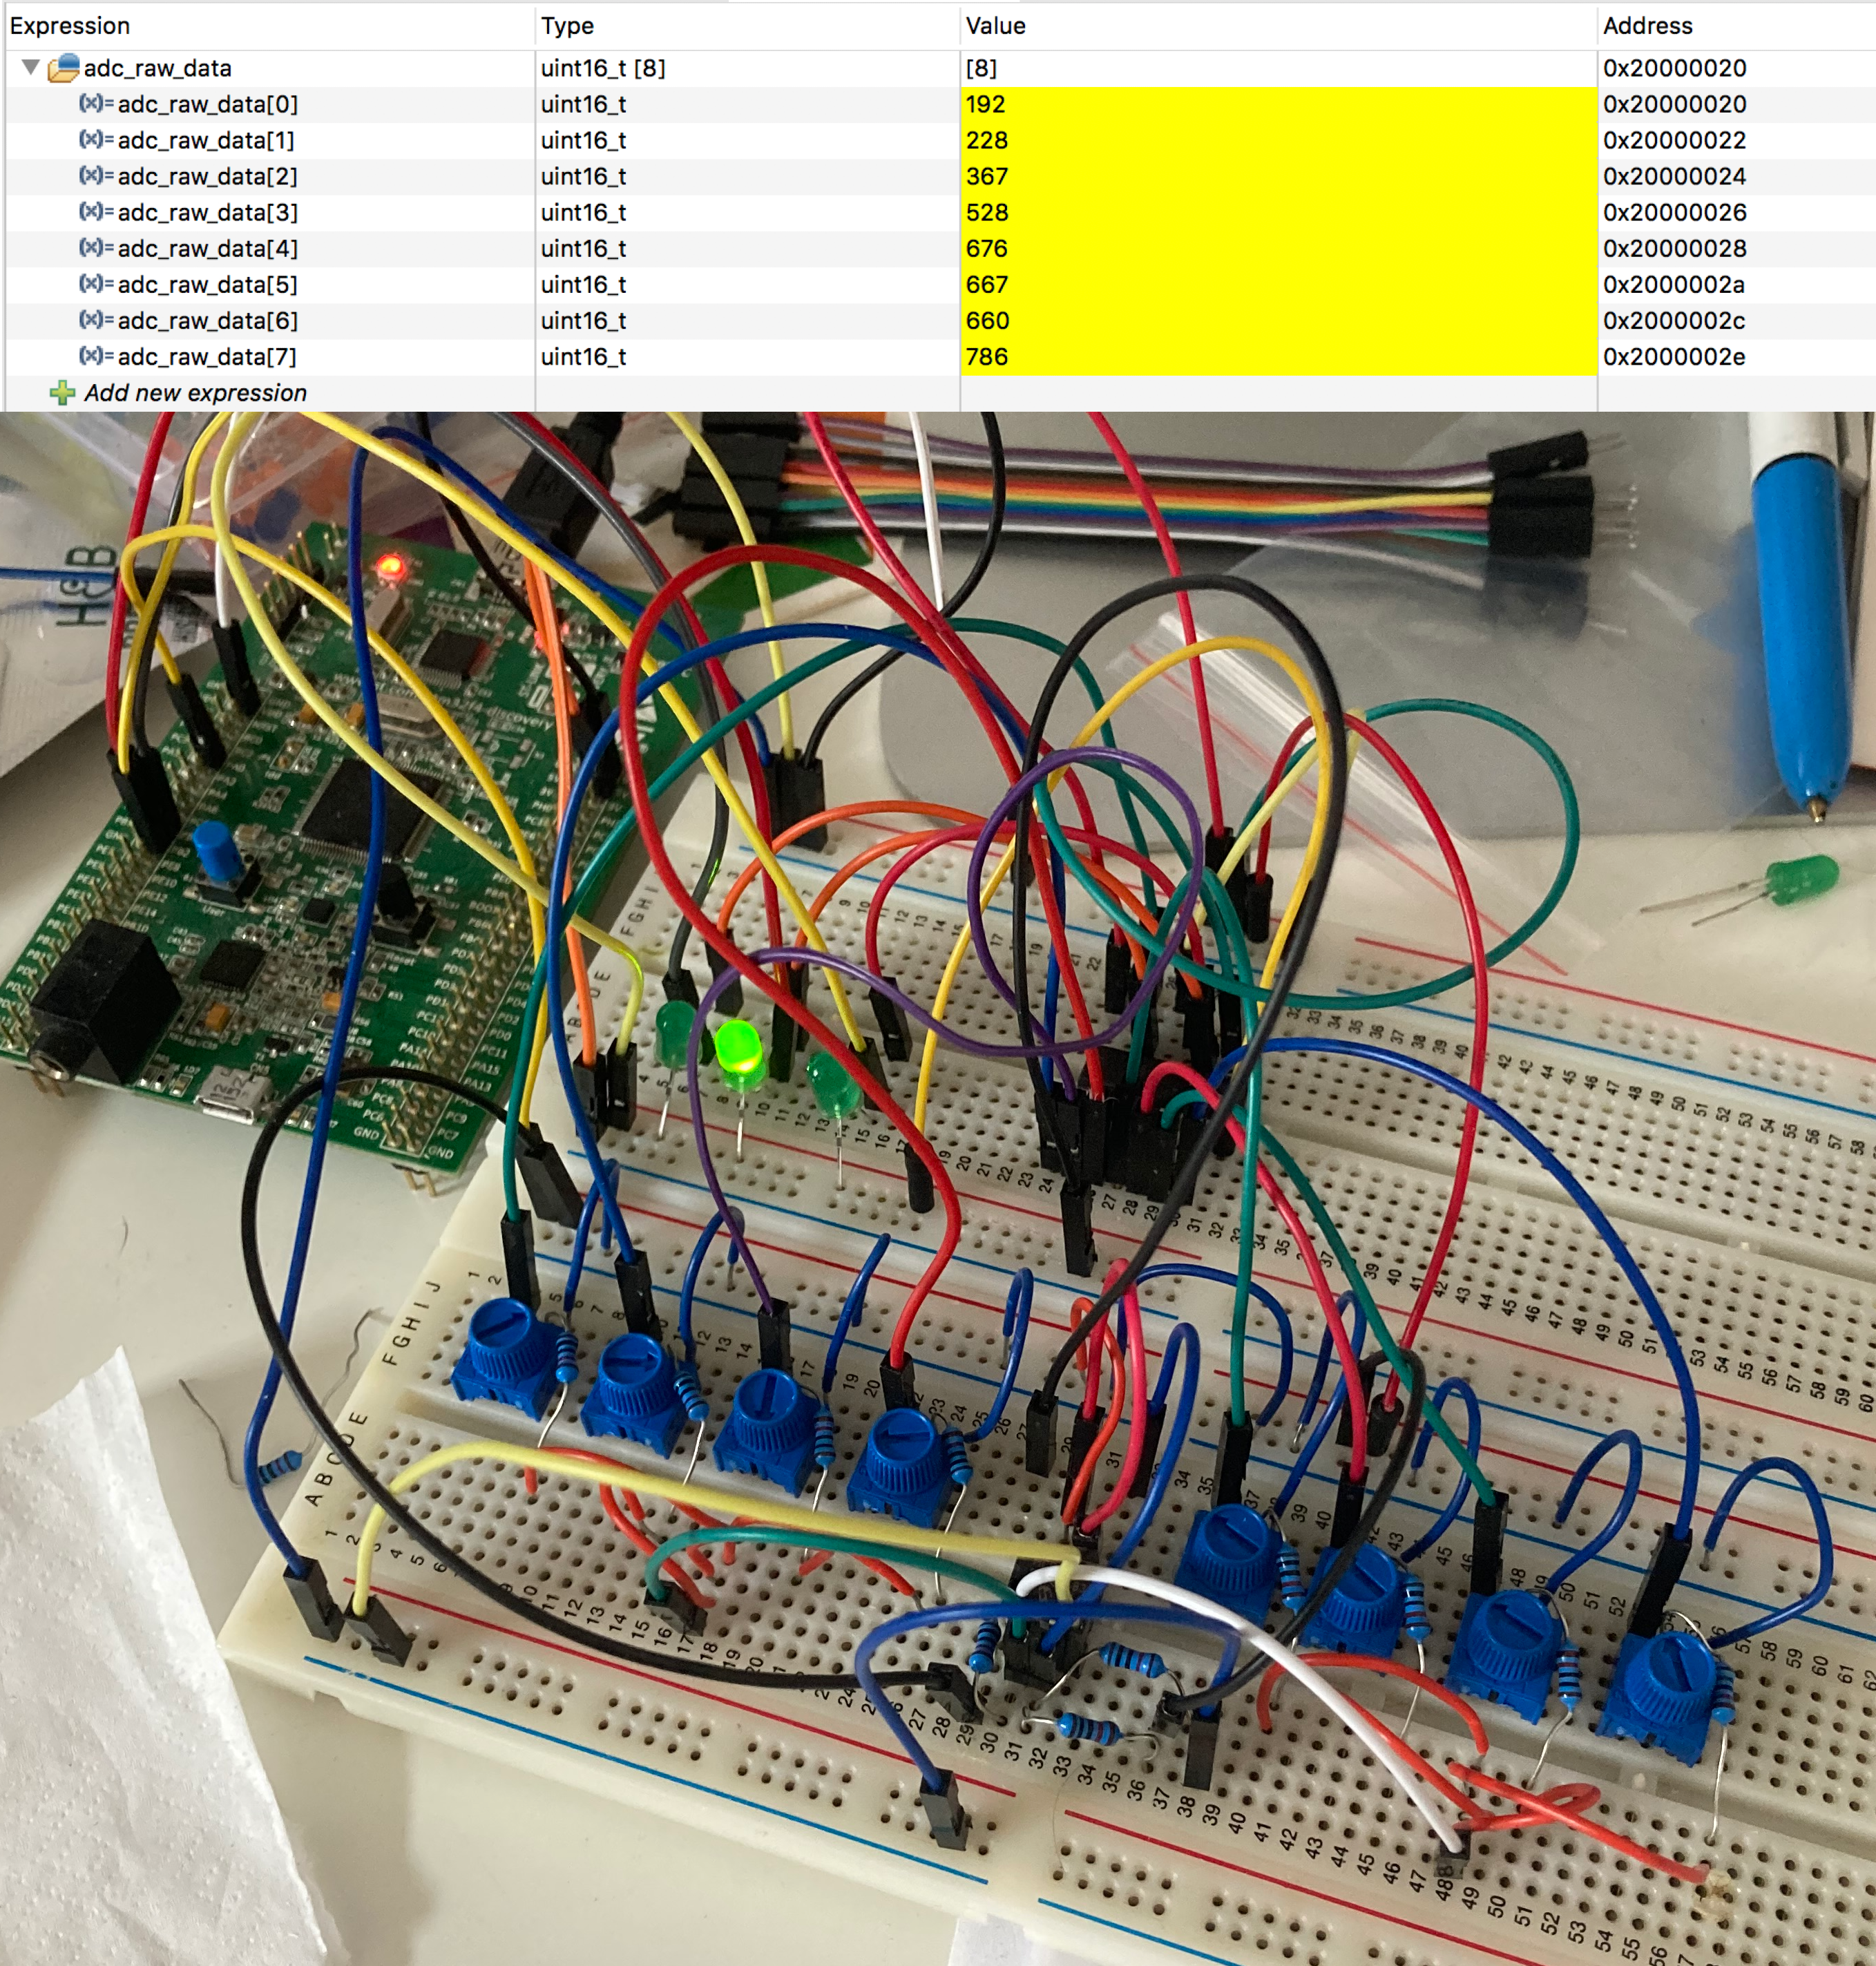
\includegraphics[width=0.85 \textwidth]{sum_amp_bread.png}}
    \caption{Testing the Summing Amplifier topology.}
    \label{fig:sum_amp_bread}
\end{figure}

\newpage
\section{Indicators}
\label{indicators}

The next step in designing the Complex Plane is to develop a method that provides real-time visual feedback for the selected grid node. As detailed in the \hyperref[appendix:hardwareinterfacing]{Hardware Interfacing} subsection of the appendix, the Complex Plane includes 64 RGB addressable LEDs. This section explains how these LEDs are programmed via SPI communication using the MCU and presents the process of reducing the memory footprint of this implementation.

\subsection{SPI Communication with the SK9822}

There are two principal types of RGB addressable LEDs: synchronous and asynchronous. A synchronous RGB addressable LED, such as the SK9822, provides complete control over frames per second and ensures accurate animations via its clock pin \cite{LED_strips}. Although more costly and power-intensive than asynchronously programmed LEDs \cite{LED_strips}, the SK9822 was deemed the more reliable option for prototyping the Complex Plane. However, if asynchronous models demonstrate sufficient speed and accuracy in reacting to node transitions, they should be considered for adoption upon commercialisation to prioritise cost and power efficiency.




To communicate with an SK9822, its data input requires precise instructions from an MCU output pin. The communication protocol is detailed in \autoref{fig:SK9822}. It starts with a four-byte frame, where all 32 bits are set to `0', followed by four bytes specifying the overall brightness and individual colour intensity levels of blue, green, and red LEDs\footnote{While the datasheet specifies the LED colour order as blue, green, and red, the correct order is actually red, blue, and green.}. The sequence concludes with a four-byte end frame, where all 32 bits are set to `1'. 

The SK9822 is designed to be programmed using a serial data structure, as illustrated in \autoref{fig:SK9823}. Each additional LED cascades to the next, so the four-byte frame specifying one LED immediately follows that of the previous LED. As a result, the final four-byte frame is sent only after all cascaded LEDs have received their respective instructions. For a chain of 64 RGB addressable LEDs, a single message consists of 264 bytes: four for the start frame, 256 for the LED frames, and four for the end frame.

\begin{figure}[H]
    \centering
    \fbox{\includegraphics[width=0.9 \textwidth]{SK9822.png}}
    \caption{SK9822 communication protocol (taken from \cite{SK9824}).}
    \label{fig:SK9822}
\end{figure}

\begin{figure}[H]
    \centering
    \fbox{\includegraphics[width=0.9 \textwidth]{SK9823.png}}
    \caption{SK9822 serial data structure (taken from \cite{SK9824}).}
    \label{fig:SK9823}
\end{figure}

\subsection{DMA-SPI Integration}

A 264-byte message is quite long for an embedded system. To efficiently send this length without burdening the CPU, an SPI peripheral in conjunction with DMA is used. This allows the message to be transferred directly from memory to the peripheral. The setup involves configuring the CPU to initiate DMA transfer by providing it with the address of the 264-byte message. The DMA then fetches this message from memory and transfers it byte by byte to the SPI peripheral autonomously. Upon completion of the transfer, the DMA sets an interrupt status flag, signalling that the transfer is complete. The Interrupt Handler, which is triggered by this status change, clears the interrupt flag to acknowledge the completion and allow the DMA to be reset and ready for the next transfer. \autoref{fig:spi} provides an illustration of this process.

\begin{figure}[ht]
    \centering
    \fbox{\includegraphics[width=0.75 \textwidth]{spi_dma.png}}
    \caption{Flowchart illustrating SPI communication with DMA functionality.}
    \label{fig:spi}
\end{figure}


\subsection{Memory Footprint Optimisation}

As detailed in the \hyperref[appendix:hardwareinterfacing]{Hardware Interfacing} subsection of the appendix, the design for the Complex Plane includes 64 RGB addressable LEDs, each capable of individual illumination in one of three modes. This configuration therefore necessitates exactly 192 unique messages. Initially, the plan was to create 192 presets, each comprising 264 bytes. Although these lengthy preset messages were transmitted successfully during testing (see \autoref{fig:led_test_1}), they do require approximately 50.7kB of memory for storage – a significant footprint for an MCU.


To optimise memory usage, a more efficient approach was implemented. By carefully examining potential four-byte combinations, five unique patterns were identified: a start frame (0x00 0x00 0x00 0x00), a red LED (0xEF 0xFF 0x00 0x00), a blue LED (0xEF 0x00 0xFF 0x00), a green LED (0xEF 0x00 0x00 0xFF), a non-lit LED (0xE0 0x00 0x00 0x00), and an end frame (0xFF 0xFF 0xFF 0xFF). By having one hard-coded buffer containing the start frame, followed by 64 non-lit LEDs and an end frame, the only additional operation required to correctly modify the message is to know the correct multiple of four-byte offsets needed to switch any of the three LED colours on or off. 

The source code in \autoref{fig:memory} illustrates the key components of a memory-efficient method for dynamically updating LED positions. To ensure that only one LED is lit at any given time, the process uses an array of preset values to manage offsets. When activating a red LED, for instance, an offset corresponding to its specific location is selected from the array, directing the update to the appropriate buffer location. Here, a non-lit LED preset is replaced with a red LED preset. After updating, the address of this buffer is sent to the DMA, which executes the transfer. Upon completion, the DMA triggers an ISR. During the ISR, the buffer is first restored to its original non-lit preset, and only afterward is the new LED position assigned to the current LED position\footnote{It is crucial that the buffer not be updated while the DMA is actively sending SPI data byte by byte, as any such changes would directly alter the ongoing transmission, inevitably leading to errors.}. This implementation significantly reduces the memory footprint from 50.7kB worth of presets to under 1kB (including the empty buffer), thereby freeing up substantial memory.

\begin{figure}[H]
    \centering
    \fbox{\includegraphics[width=0.65 \textwidth]{led_test_1.jpg}}
    \caption{Testing the indicator driver using presets of 264-byte length.}
    \label{fig:led_test_1}
\end{figure}



\begin{figure}[H]
    \centering
    \fbox{\includegraphics[width=0.95 \textwidth]{memory.png}}
    \caption{Source code for memory-efficient  LED driver.}
    \label{fig:memory}
\end{figure}
















\newpage
\section{Wiring}
\label{wiring}
This section presents two contrasting wiring approaches – software-centric and hardware-centric – and explores their roles in effectively managing node transitions on the Complex Plane. Initially, the discussion centres on the algorithms designed to ensure accurate node transitions, with distinct algorithms handling horizontal, vertical, and rotational movements. It then examines the decision-making process that integrates both wiring approaches during the PCB design phase of the Complex Plane. Following the completion of the PCB, a test of the entire sensor and indicator system is conducted.

\subsection{Node Transition Algorithms}

To implement the functions for the X, Y, and C clocks on the Complex Plane, it is necessary to develop a specific algorithm for each function. This involves dividing the Complex Plane into four quadrants, each containing four rows and four columns. By identifying the current quadrant, row, and column of a particular node, an algorithm can be designed to enable the node to transition to the next position – horizontally, vertically, or rotationally anti-clockwise (see \autoref{fig:node_transitions} for the source code implementation of these algorithms).  

\subsubsection{Horizontal Transition}

The horizontal transition algorithm calculates the next position of a node by moving it horizontally from left to right within the same quadrant. If the node is at the last column of a row, it wraps around to the first column of the same row. 

\subsubsection{Vertical Transition}

The vertical transition algorithm moves the node vertically from the bottom to the top within the same quadrant. It calculates the next row position, and if the node is at the top of the quadrant, it wraps around to the bottom row while keeping the column constant.

\subsubsection{Rotational Transition}
The rotational transition algorithm facilitates the movement of a node to an adjacent quadrant in an anti-clockwise direction, akin to the mathematical `i' operator in complex number multiplication. This movement adjusts the node's position to the new quadrant, ensuring the correct transition across quadrant boundaries.

\begin{figure}[H]
    \centering
    \fbox{\includegraphics[width=0.9 \textwidth]{node_transitions.png}}
    \caption{Source code implementation of the node transition algorithms.}
    \label{fig:node_transitions}
\end{figure}


\newpage

\subsection{Software-centric Wiring}

The presented algorithms manage the correct transitions from the current node to the next by organising the SPI addresses of the RGB addressable LEDs (discussed in the \hyperref[indicators]{Indicators} section) in a particular sequence. This sequence is defined here as software-centric wiring. 

The software-centric wiring sequence of the LEDs, as illustrated on the left-hand side of \autoref{fig:RGB_wiring}, starts at the top-left quadrant. It systematically scans across the columns of each row, moving from left to right, and proceeds downward row by row within the quadrant. Upon completing all rows in the quadrant, the sequence advances to the next quadrant following an anti-clockwise direction. Initially, the wiring seemed appropriate, fully compatible with the implemented algorithms. However, during the PCB design for the Complex Plane, it became evident that an alternative wiring approach was necessary to achieve optimal results.


\begin{figure}[H]
    \centering
    \fbox{\includegraphics[width=0.9 \textwidth]{RGB_wiring.png}}
    \caption{Software-centric and hardware-centric wirings of the cascaded LED chain.}
    \label{fig:RGB_wiring}
\end{figure}

\subsection{Hardware-centric Wiring}
When initially adopting the software-centric wiring approach during PCB development, it became evident that this method would result in suboptimal design outcomes. An examination of the PCB design in \autoref{fig:SK9822_wiring} sheds light on the matter.

\begin{figure}[H]
    \centering
    \fbox{\includegraphics[width=0.95 \textwidth]{SK9822_wiring.png}}
    \caption{Close-up of the PCB design of the Complex Plane.}
    \label{fig:SK9822_wiring}
\end{figure}

Had the software-centric wiring been adopted when designing the PCB, it would have featured an excessive number of vias, as this wiring method would interfere with the power line and MUX traces. This would not only complicate the trace routing, making it awkwardly laid out, but also reduce the area of the ground plane. Conversely, by opting for the snake-patterned hardware-centric wiring approach (shown in \autoref{fig:RGB_wiring} and highlighted in \autoref{fig:SK9822_wiring}), the power lines are elegantly arranged, and the number of vias is minimised. \autoref{fig:3V} and \autoref{fig:5V} show the benefits of adopting a hardware-centric wiring approach. The power lines are laid out neatly and in a symmetrical fashion, and the ground plane area is mostly reduced at the outer edges of the PCB, electrically far away from sensitive circuitry.

Given the advantages of the hardware-centric wiring for the PCB, it has been adopted. However, the SPI addresses of the LEDs needed to be reordered to emulate the software-centric wiring, effectively creating a hybrid approach that resolves the dilemma\footnote{In retrospect, prioritising the physical neatness and symmetry of the MUX wiring over strict adherence to the datasheet’s sensor assignments could have been equally advantageous. This approach would have improved wire management on the PCB, while still allowing for rearrangement of sensor input mappings in software to maintain system functionality.}. This strategy not only ensures a superior PCB design but also accommodates the existing algorithmic framework. \autoref{fig:mapping} contains source code that demonstrates the required reordering of the LED addresses.


\begin{figure}[H]
    \centering
    \fbox{\includegraphics[width=0.65 \textwidth]{3V.png}}
    \caption{Highlighting the 3V power lines of the PCB.}
    \label{fig:3V}
\end{figure}


\begin{figure}[H]
    \centering
    \fbox{\includegraphics[width=0.65 \textwidth]{5V.png}}
    \caption{Highlighting the 5V power lines of the PCB.}
    \label{fig:5V}
\end{figure}

\begin{figure}[H]
    \centering
    \fbox{\includegraphics[width=0.55 \textwidth]{mapping.png}}
    \caption{Mapping the SPI presets.}
    \label{fig:mapping}
\end{figure}

\subsection{System Test}

After the PCB for the Complex Plane was designed and assembled, the sensor and indicator system underwent testing. A single test can evaluate both the sensor and indicator systems by activating a node transition algorithm during the ISR of the DMA tasked with transferring and storing all sensor readings in memory\footnote{It should be noted that the DMA’s ISR is triggered not by the transfer of a single sensor reading, but by the complete transfer of the entire sensor network to memory.}. \autoref{fig:system_test} illustrates the test conducted and effectively demonstrates the system's functionality.


\begin{figure}[H]
    \centering
    \fbox{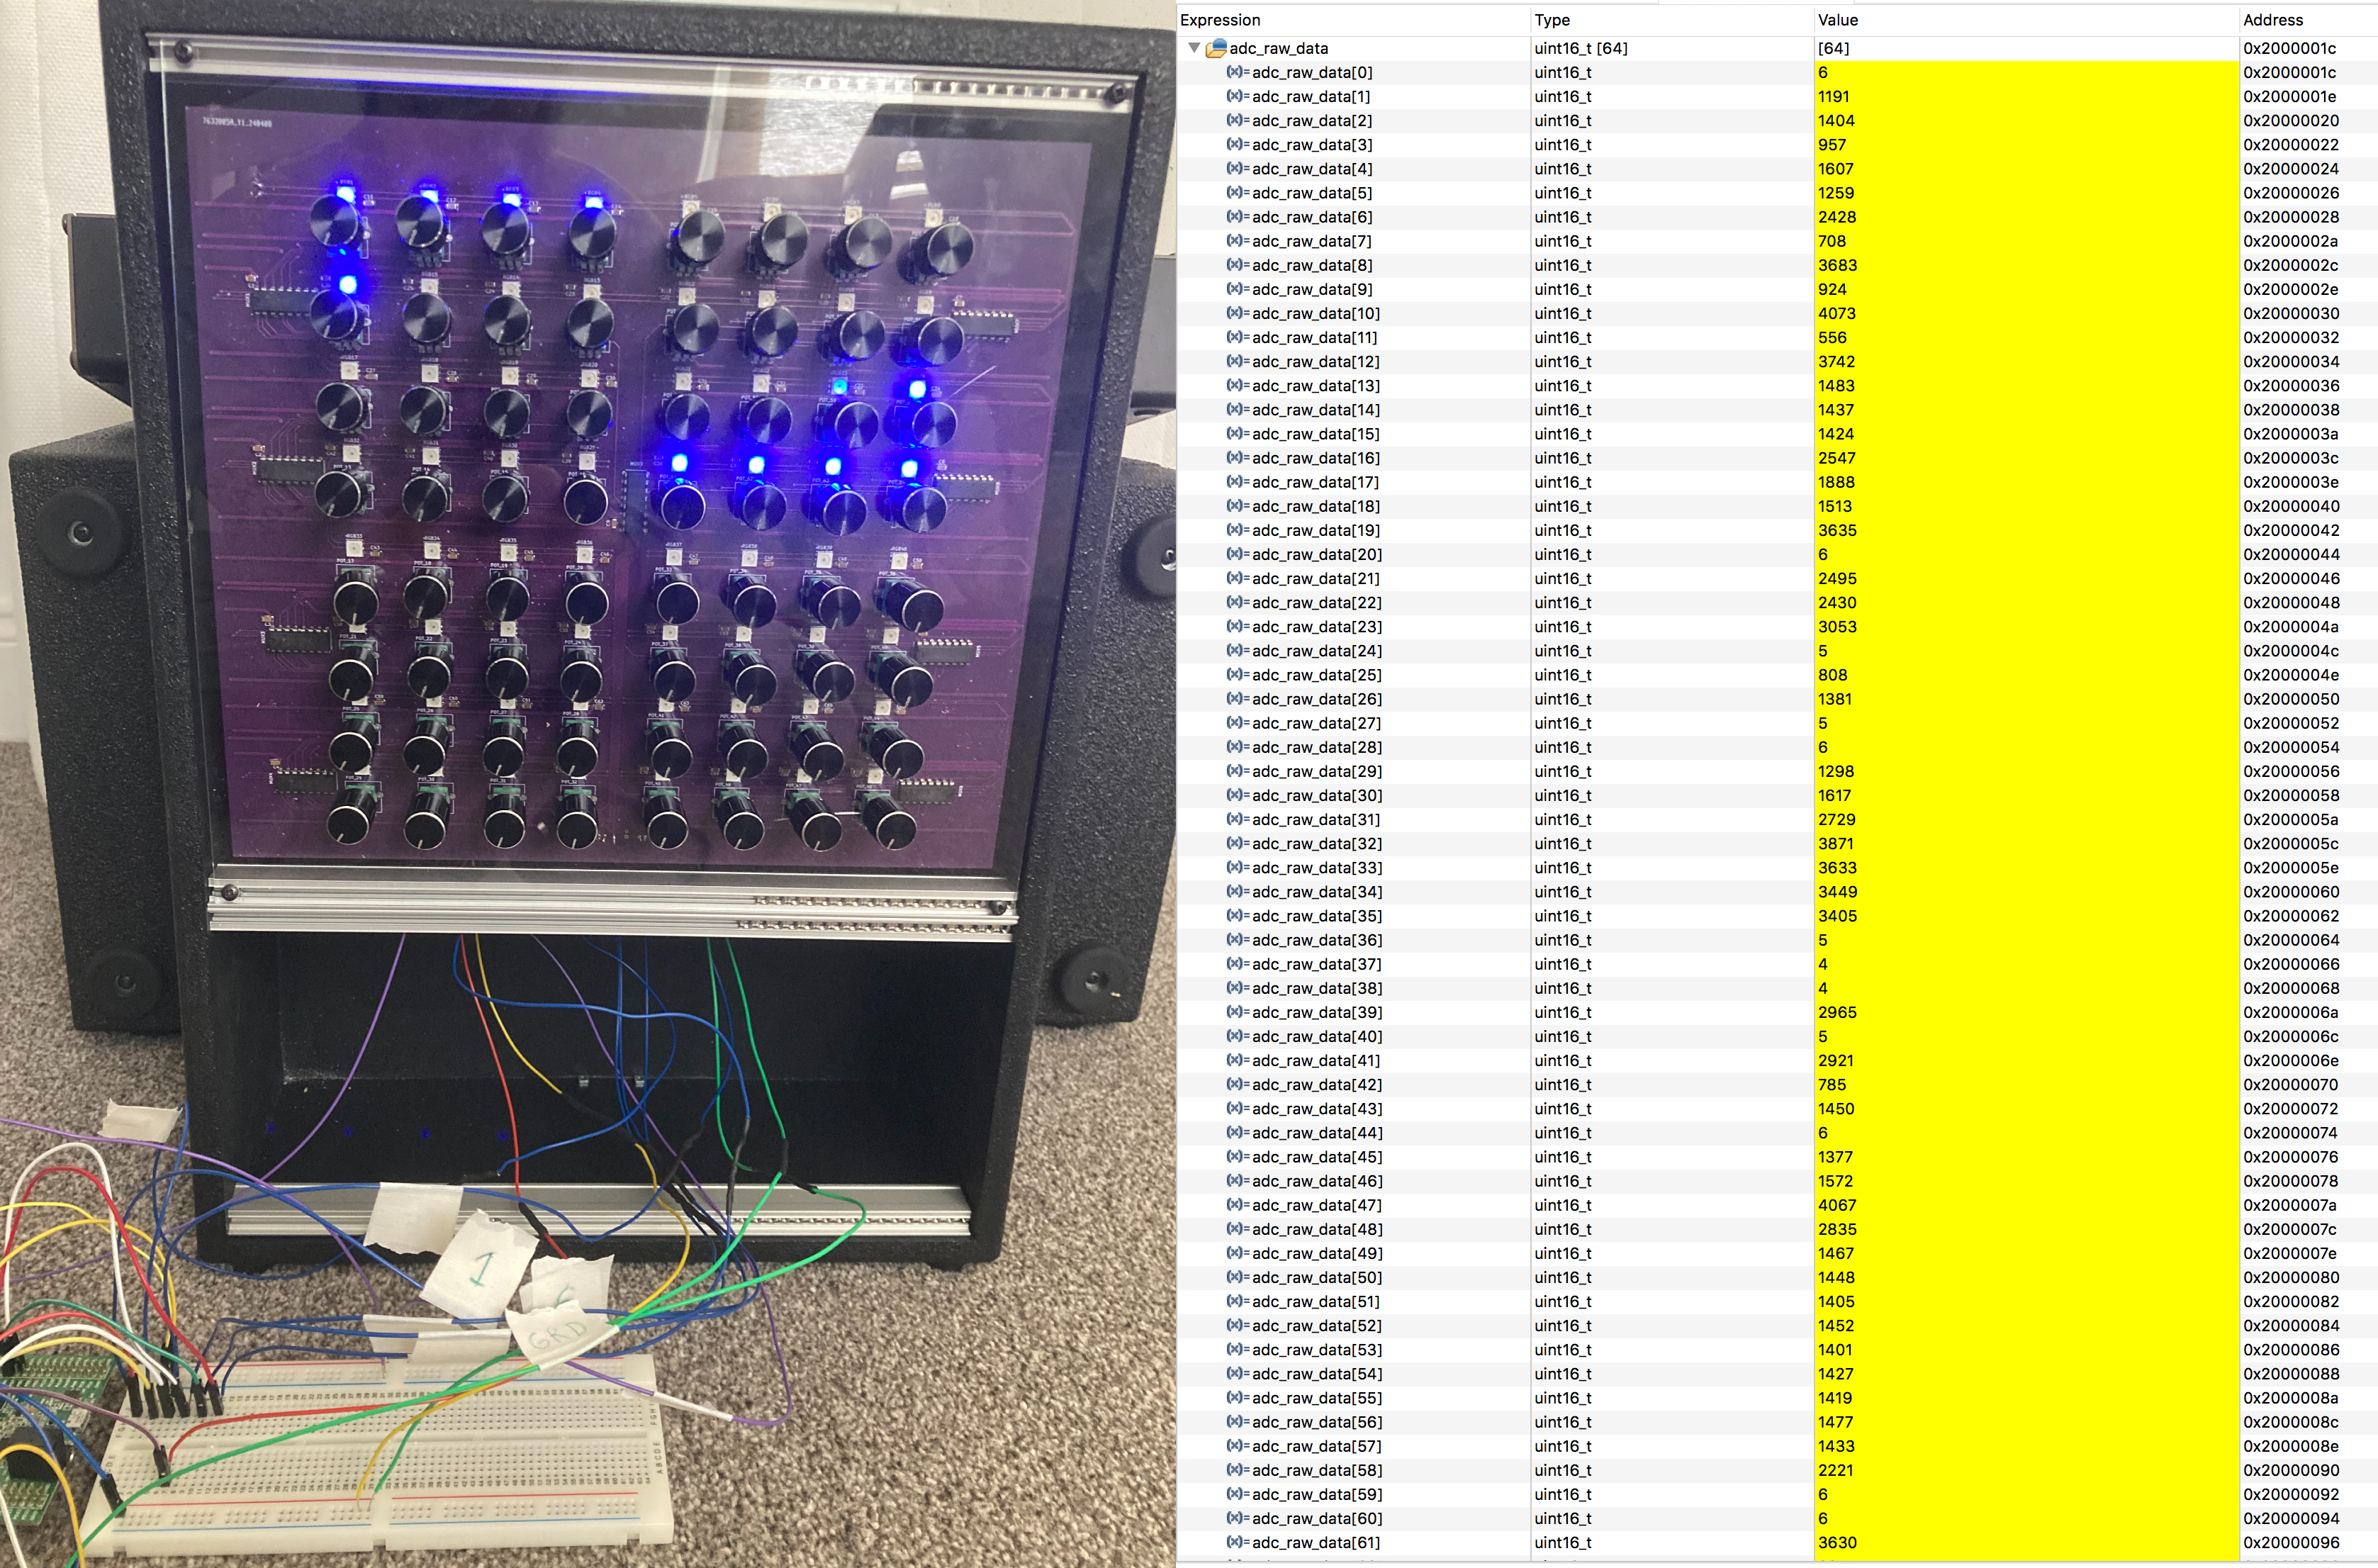
\includegraphics[width=0.9 \textwidth]{system_test.png}}
    \caption{Testing the sensor and indicator system.}
    \label{fig:system_test}
\end{figure}















\newpage

\section{Ergonomics}

This section deals with ergonomics in product design. It argues the advantage of choosing a three-way switch over three separate push buttons for selecting between three LED colours – aiming to streamline user interactions and reduce cognitive load. The technical specifics of using a Double-Pole Double-Throw (DPDT) ON–ON–ON switch are detailed, alongside a discussion of a more cost-effective alternative that employs a Single-Pole Double-Throw (SPDT) ON–OFF–ON switch. The final part of this section addresses ergonomic considerations related to the user interface of the sequencer.


\subsection{Push Buttons}

It is documented in the \hyperref[appendix:hardwareinterfacing]{Hardware Interfacing} subsection of the appendix that the Complex Plane should feature three colour-coded modes. These modes correspond to the X, Y, and C clock configurations of the recurring decimal algorithm, as detailed in the \hyperref[appendix:recurringdecimals]{Rhythm Generation via Recurring Decimals} subsection of the appendix. Although various approaches to mode selection exist, the most straightforward method during the prototyping phase involves using three push buttons.

Each button connects to a designated input pin on the MCU, enabling the switch to the corresponding mode. To enhance efficiency, the system employs External Interrupts (EXTIs) instead of having the CPU continuously poll the state of the MCU's input pins. This configuration allows each pin to trigger an interrupt when a falling edge is detected, prompting the CPU to update the mode status in the program\footnote{This technique was also used for manually triggering the X, Y, and C node transitions on the Complex Plane but was not detailed earlier to avoid repetition.}. 

Due to the mechanical bouncing effects of button presses, multiple interrupts can be triggered, leading to unnecessary CPU interruptions and unreliable performance. To mitigate this, a combination of hardware and software debouncing strategies is implemented. Simple RC circuitry, consisting of a \SI{10}{\kilo\ohm} resistor in series with the button and a \SI{100}{\nano\farad} capacitor connected from the junction point to ground, is introduced between the push button and the MCU to filter out high-frequency components associated with bouncing. Complementing this, the SysTick Timer – a timer built into the microprocessor – is employed to introduce a delay after the initial button press is detected. This delay prevents the processing of subsequent signals, ensuring that only the first stable activation is recognised. \autoref{fig:EXTI} contains the source code essential for the mode selection functionality per EXTI line, while \autoref{fig:button} presents the breadboarding setup, confirming its operational success.

\begin{figure}[H]
    \centering
    \fbox{\includegraphics[width=0.95 \textwidth]{EXTI_code.jpg}}
    \caption{Source code for mode selection driver.}
    \label{fig:EXTI}
\end{figure}


\begin{figure}[H]
    \centering
    \fbox{
\includegraphics[width=0.95 \textwidth]{button_test.jpg}}
    \caption{Testing the button switches.}
    \label{fig:button}
\end{figure}



\subsection{Three-way Switch}

From a functional standpoint, using a dedicated button to select the mode of the Complex Plane is adequate. However, this approach introduces an excessive number of peripherals for the user, potentially increasing cognitive load during operation. A more ergonomic solution involves a mechanism for switching between modes, reflecting the principle that there is no need to select more than one mode at a time or to repeatedly select the same mode once activated. This ergonomic principle is evident in many synthesisers, particularly the Korg Minilogue, which features not only three-way but also four and five-way switches\footnote{In the Minilogue, the four and five-way switches are programmable rather than mechanical. They enable users to increment and decrement the selected mode, with indicator LEDs included to signify the selected mode's activation.}, as shown in \autoref{fig:minilogue}.

\begin{figure}[H]
    \centering
    \fbox{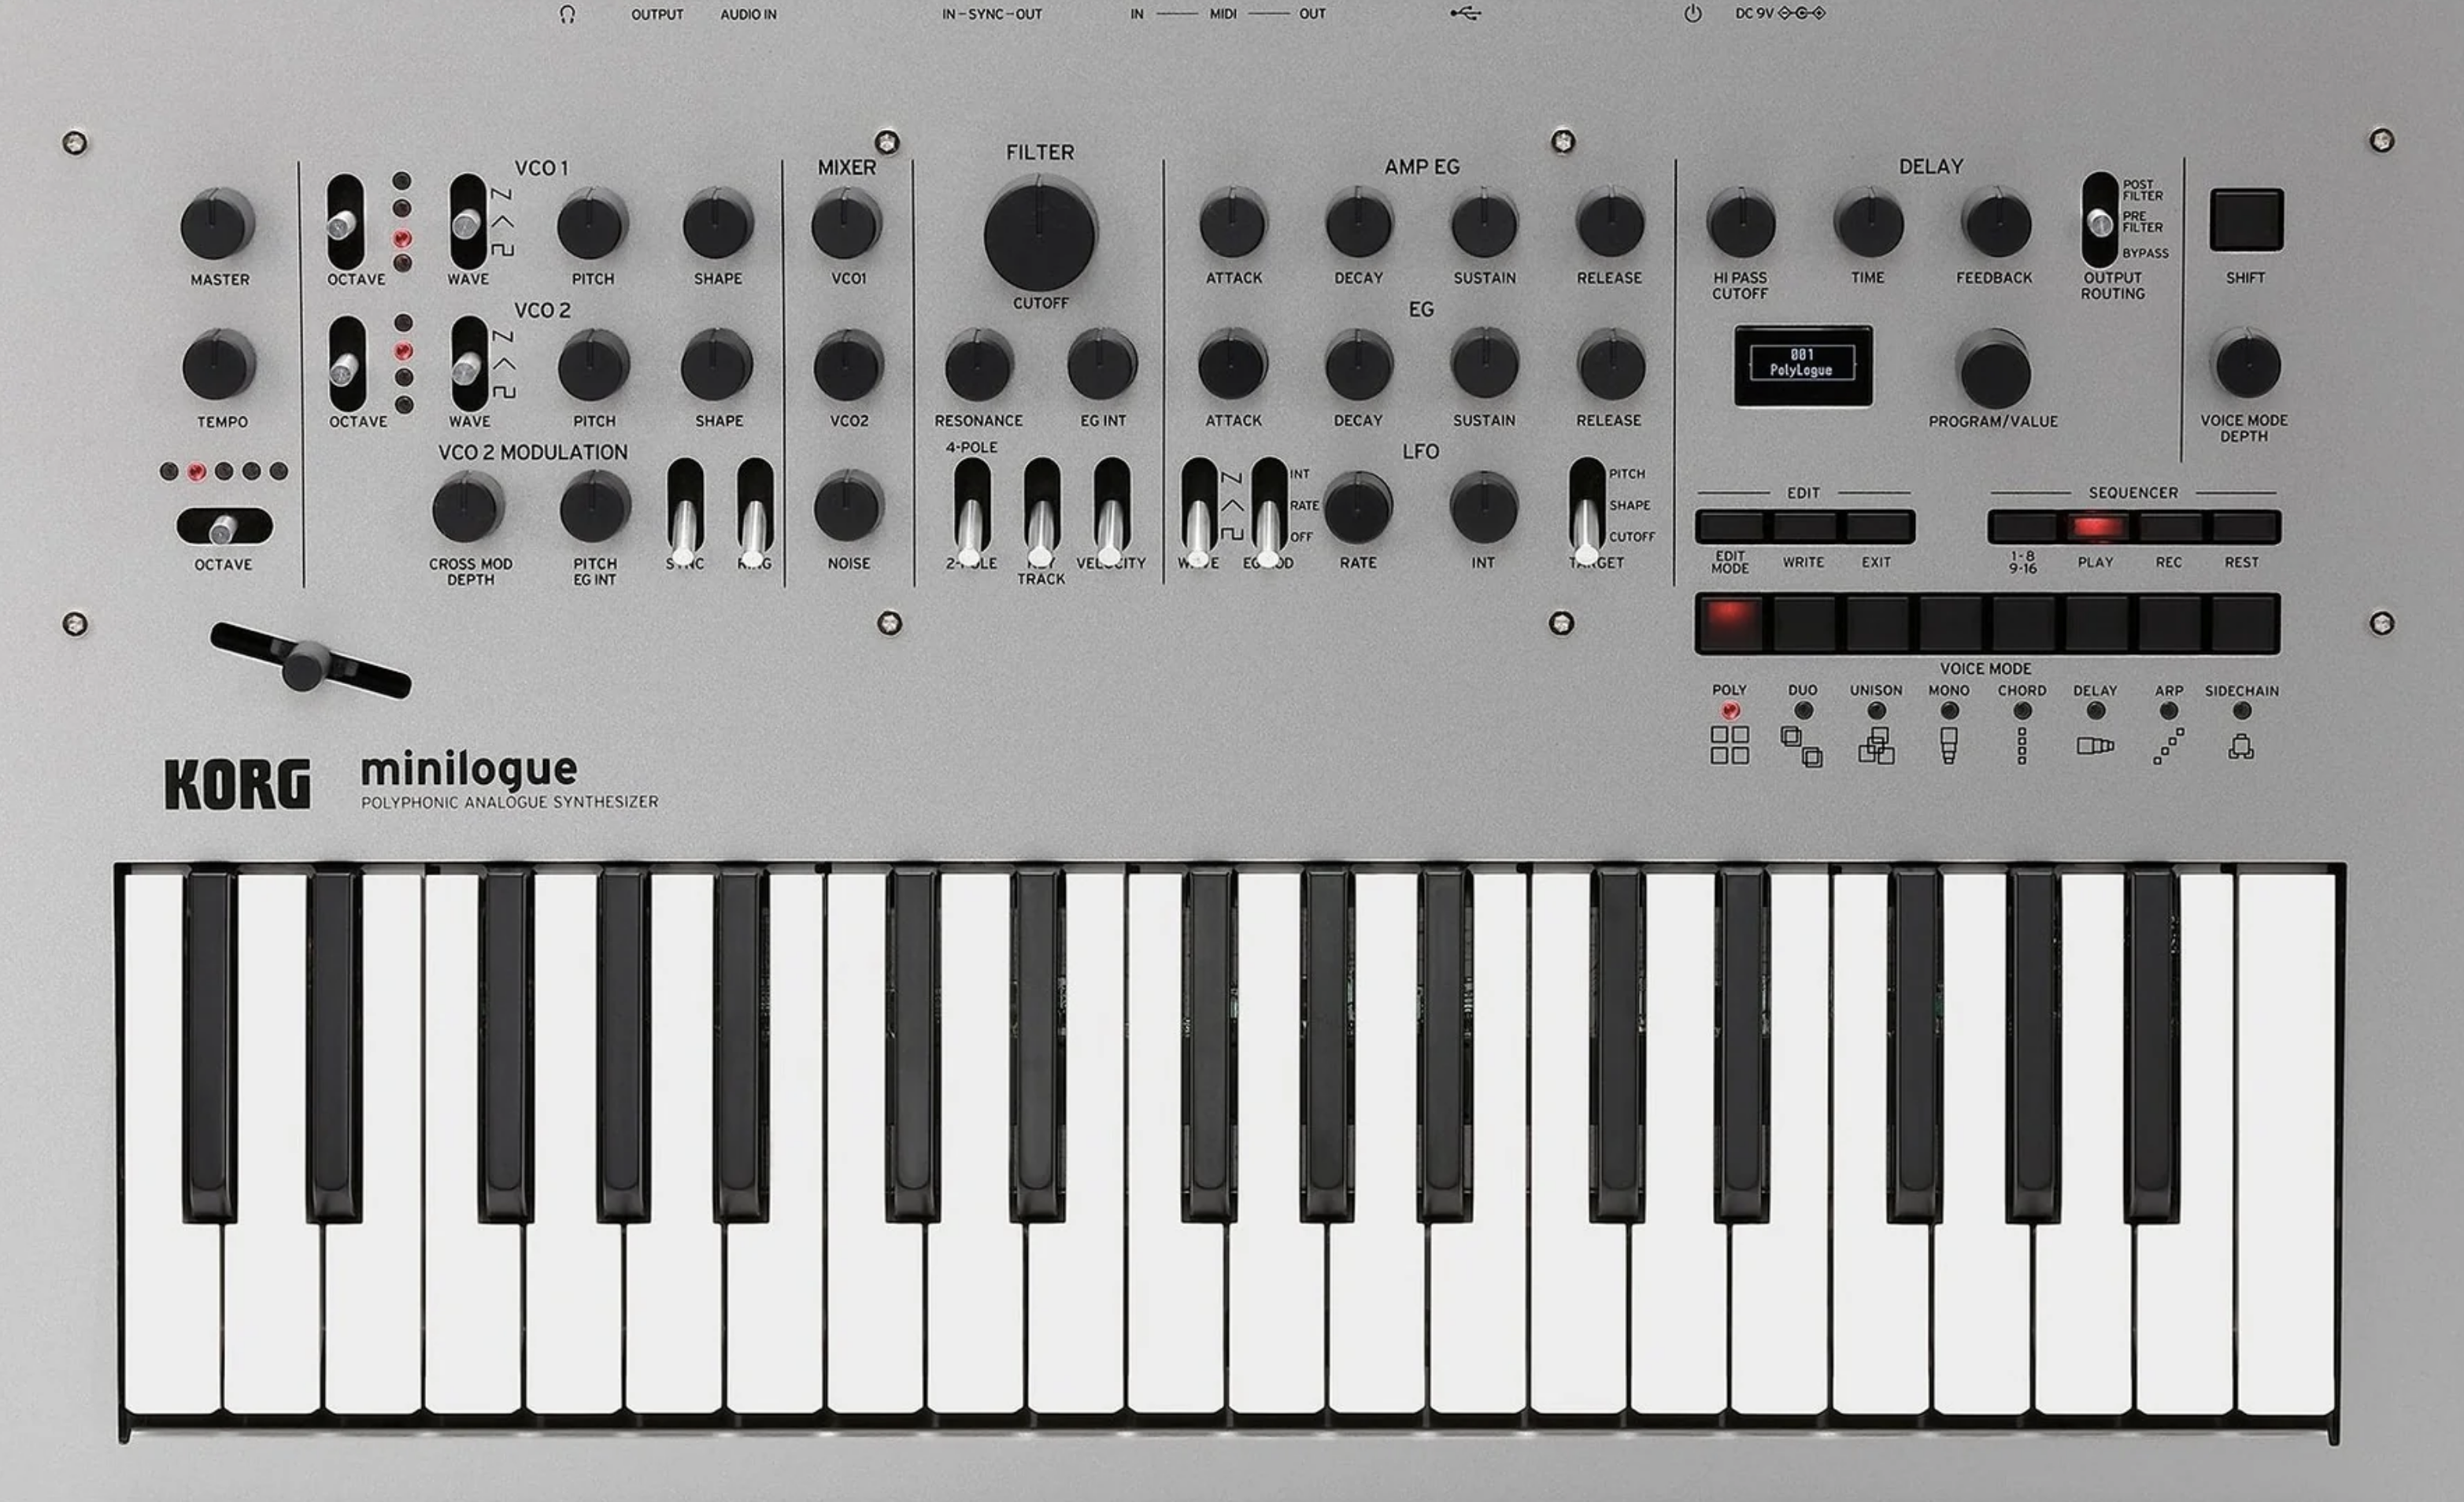
\includegraphics[width=0.8 \textwidth]{minilogue.png}}
    \caption{Korg Minilogue synthesiser (taken from \cite{minilogue}).}
    \label{fig:minilogue}
\end{figure}


A practical method for achieving three-way switching functionality – without resorting to the generally more bulky and expensive rotary selectors – involves using a DPDT ON-ON-ON switch, as demonstrated in \autoref{fig:SP3T}. In the diagram, each circle represents a pin of the switch, and the dashed line indicates the wiring required for three-way operation. The solid lines show the internal connections specific to each switch position, while each colour pattern illustrates the routing corresponding to these positions. As demonstrated in \autoref{fig:DPDT}, this configuration offers the same functionality as the push buttons but with enhanced ergonomic benefits.


\begin{figure}[H]
    \centering
    \fbox{\includegraphics[width=0.9 \textwidth]{SP3T.png}}
    \caption{DPDT ON-ON-ON switch configured as a three-way switch.}
    \label{fig:SP3T}
\end{figure}

\begin{figure}[H]
    \centering
    \fbox{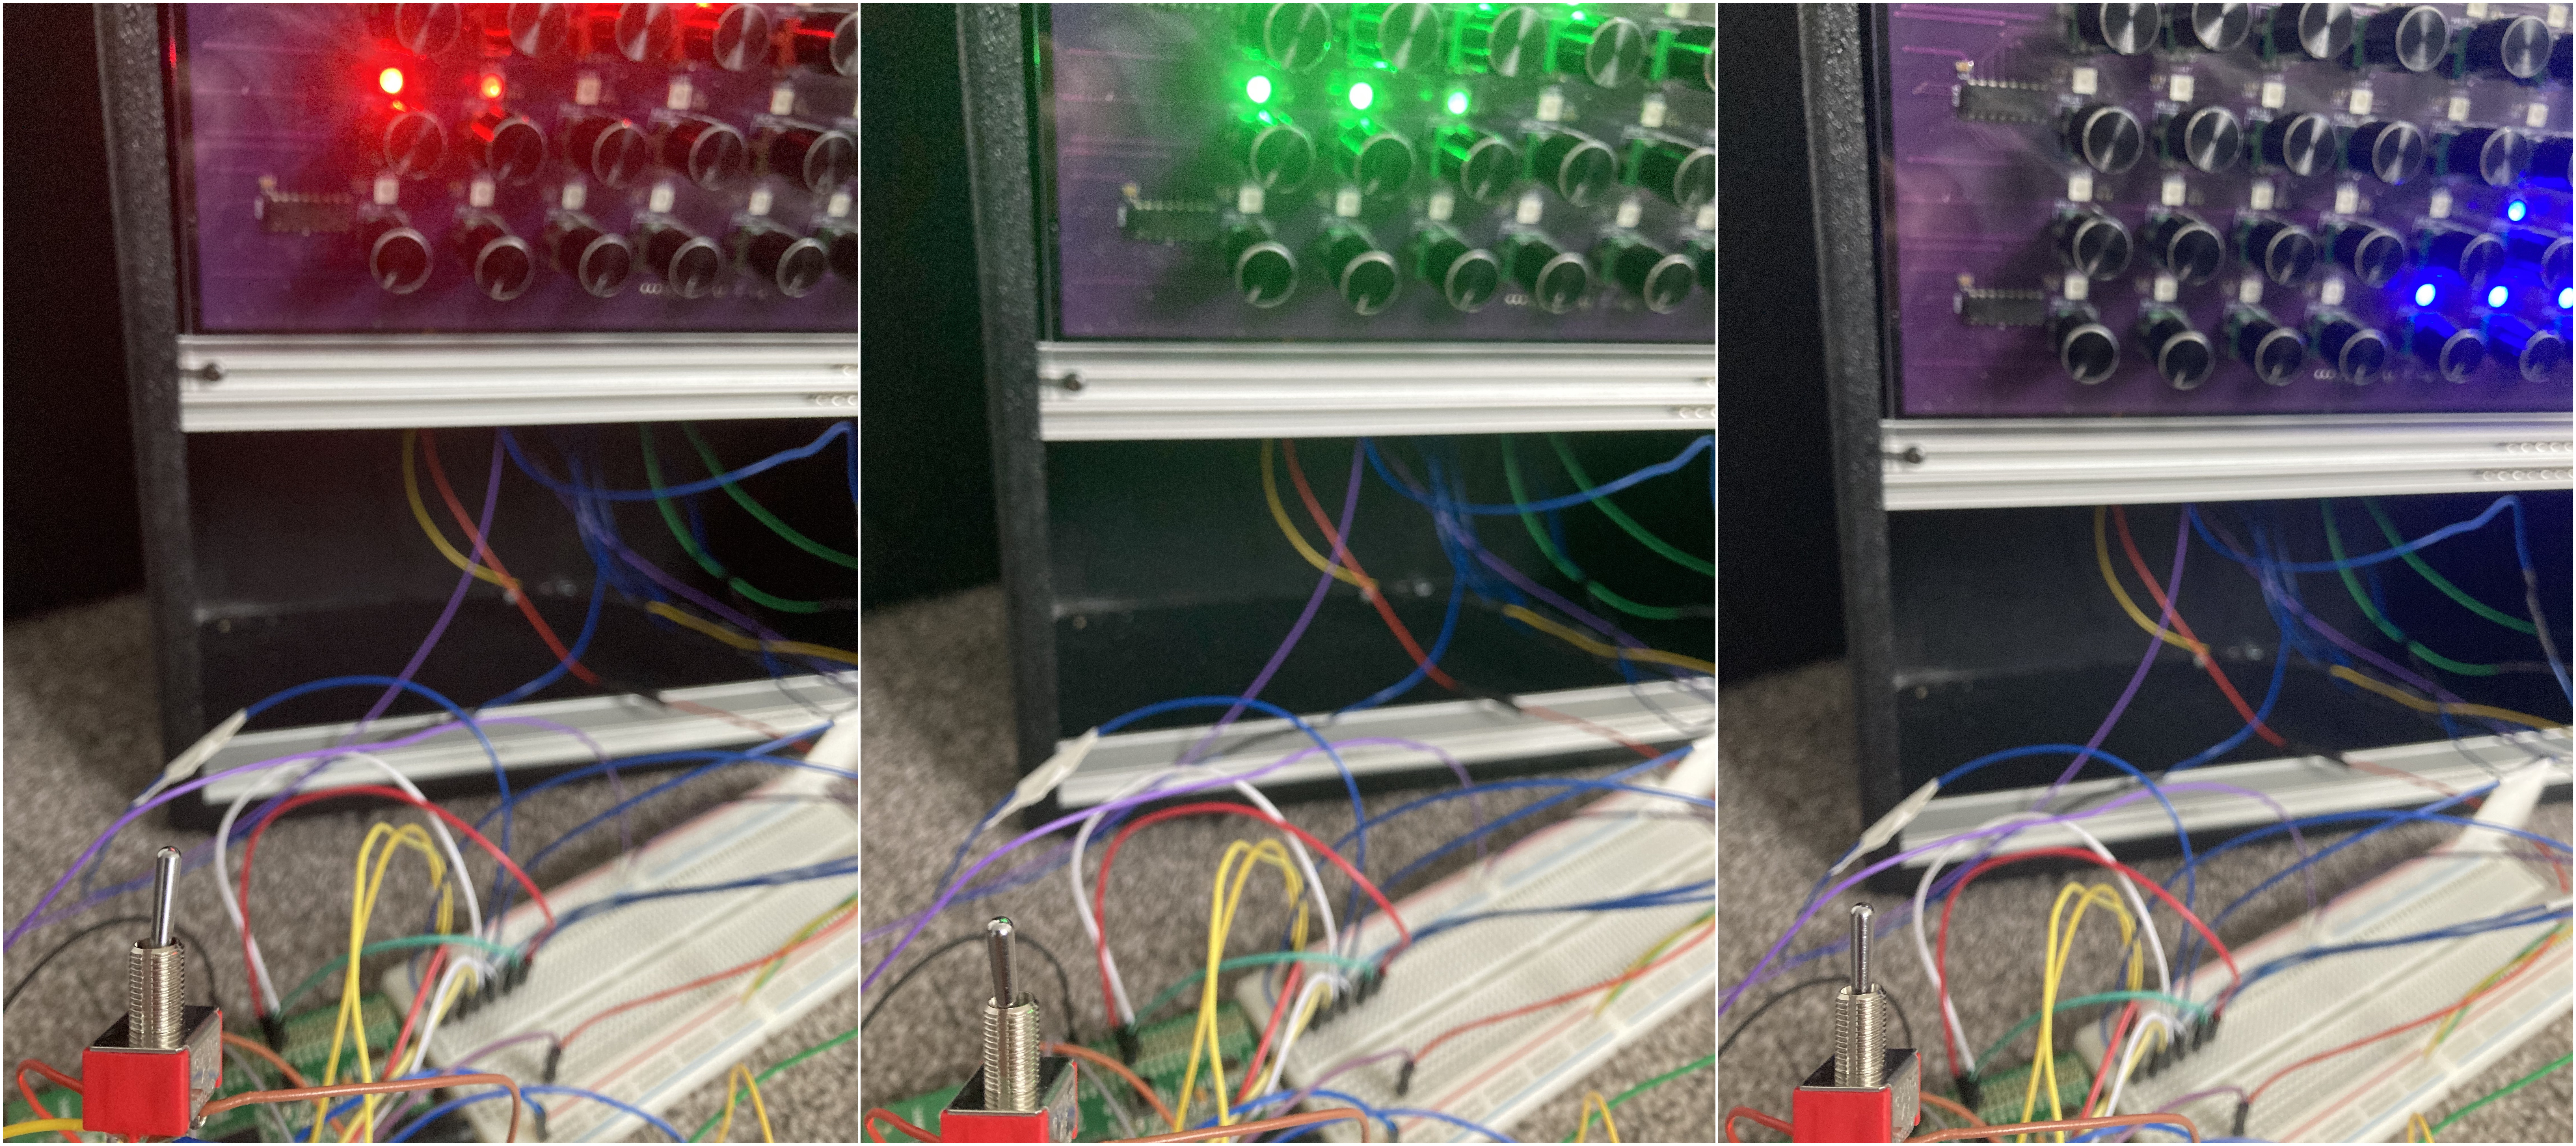
\includegraphics[width=0.9 \textwidth]{DPDT_test.jpg}}
    \caption{Testing the DPDT as a three-way switch.}
    \label{fig:DPDT}
\end{figure}


While the DPDT ON-ON-ON switch is ideal for analog input signals, a more cost-effective option should be considered for constant digital signals, as in this setup.  An SPDT ON-OFF-ON switch integrated with the MCU reduces hardware complexity and costs by using a more basic switch type. 

As shown in \autoref{fig:SPDT}, each of the SPDT switch's outer terminals is connected to both VCC and separate input pins on the MCU, set to use internal pull-down resistors. This configuration ensures that when neither terminal is connected to VCC (in the OFF position), both input pins register LOW (0). Conversely, when one terminal is connected to VCC, the corresponding input pin registers HIGH (1), while the other remains LOW. This configuration allows the MCU to distinguish between three distinct states by using a switch-case statement to evaluate the resultant binary value\footnote{Note that the EXTIs must be configured to trigger on both rising and falling edges for this to function properly.}. Thus, this setup is functionally and ergonomically equivalent to the DPDT configuration yet costs less and requires one less input pin and EXTI line. The source code necessary to enable such functionality is shown in \autoref{fig:SPDT_code} while confirmation that it works is shown in \autoref{fig:SPDT_test}\footnote{The designer searched for a SPDT ON-OFF-ON switch in the University labs, but this component was not available. Instead, a DPDT ON-ON-ON switch was used and configured to replicate the functionality of the required SPDT switch. Refer to \autoref{fig:DPDT_to_SPDT} for the wiring diagram that illustrates how this adaptation was achieved.}.

\begin{figure}[H]
    \centering
    \fbox{\includegraphics[width=0.95 \textwidth]{SPDT.png}}
    \caption{SPDT ON-OFF-ON switch as a three-way switch.}
    \label{fig:SPDT}
\end{figure}


\begin{figure}[ht]
    \centering
    \fbox{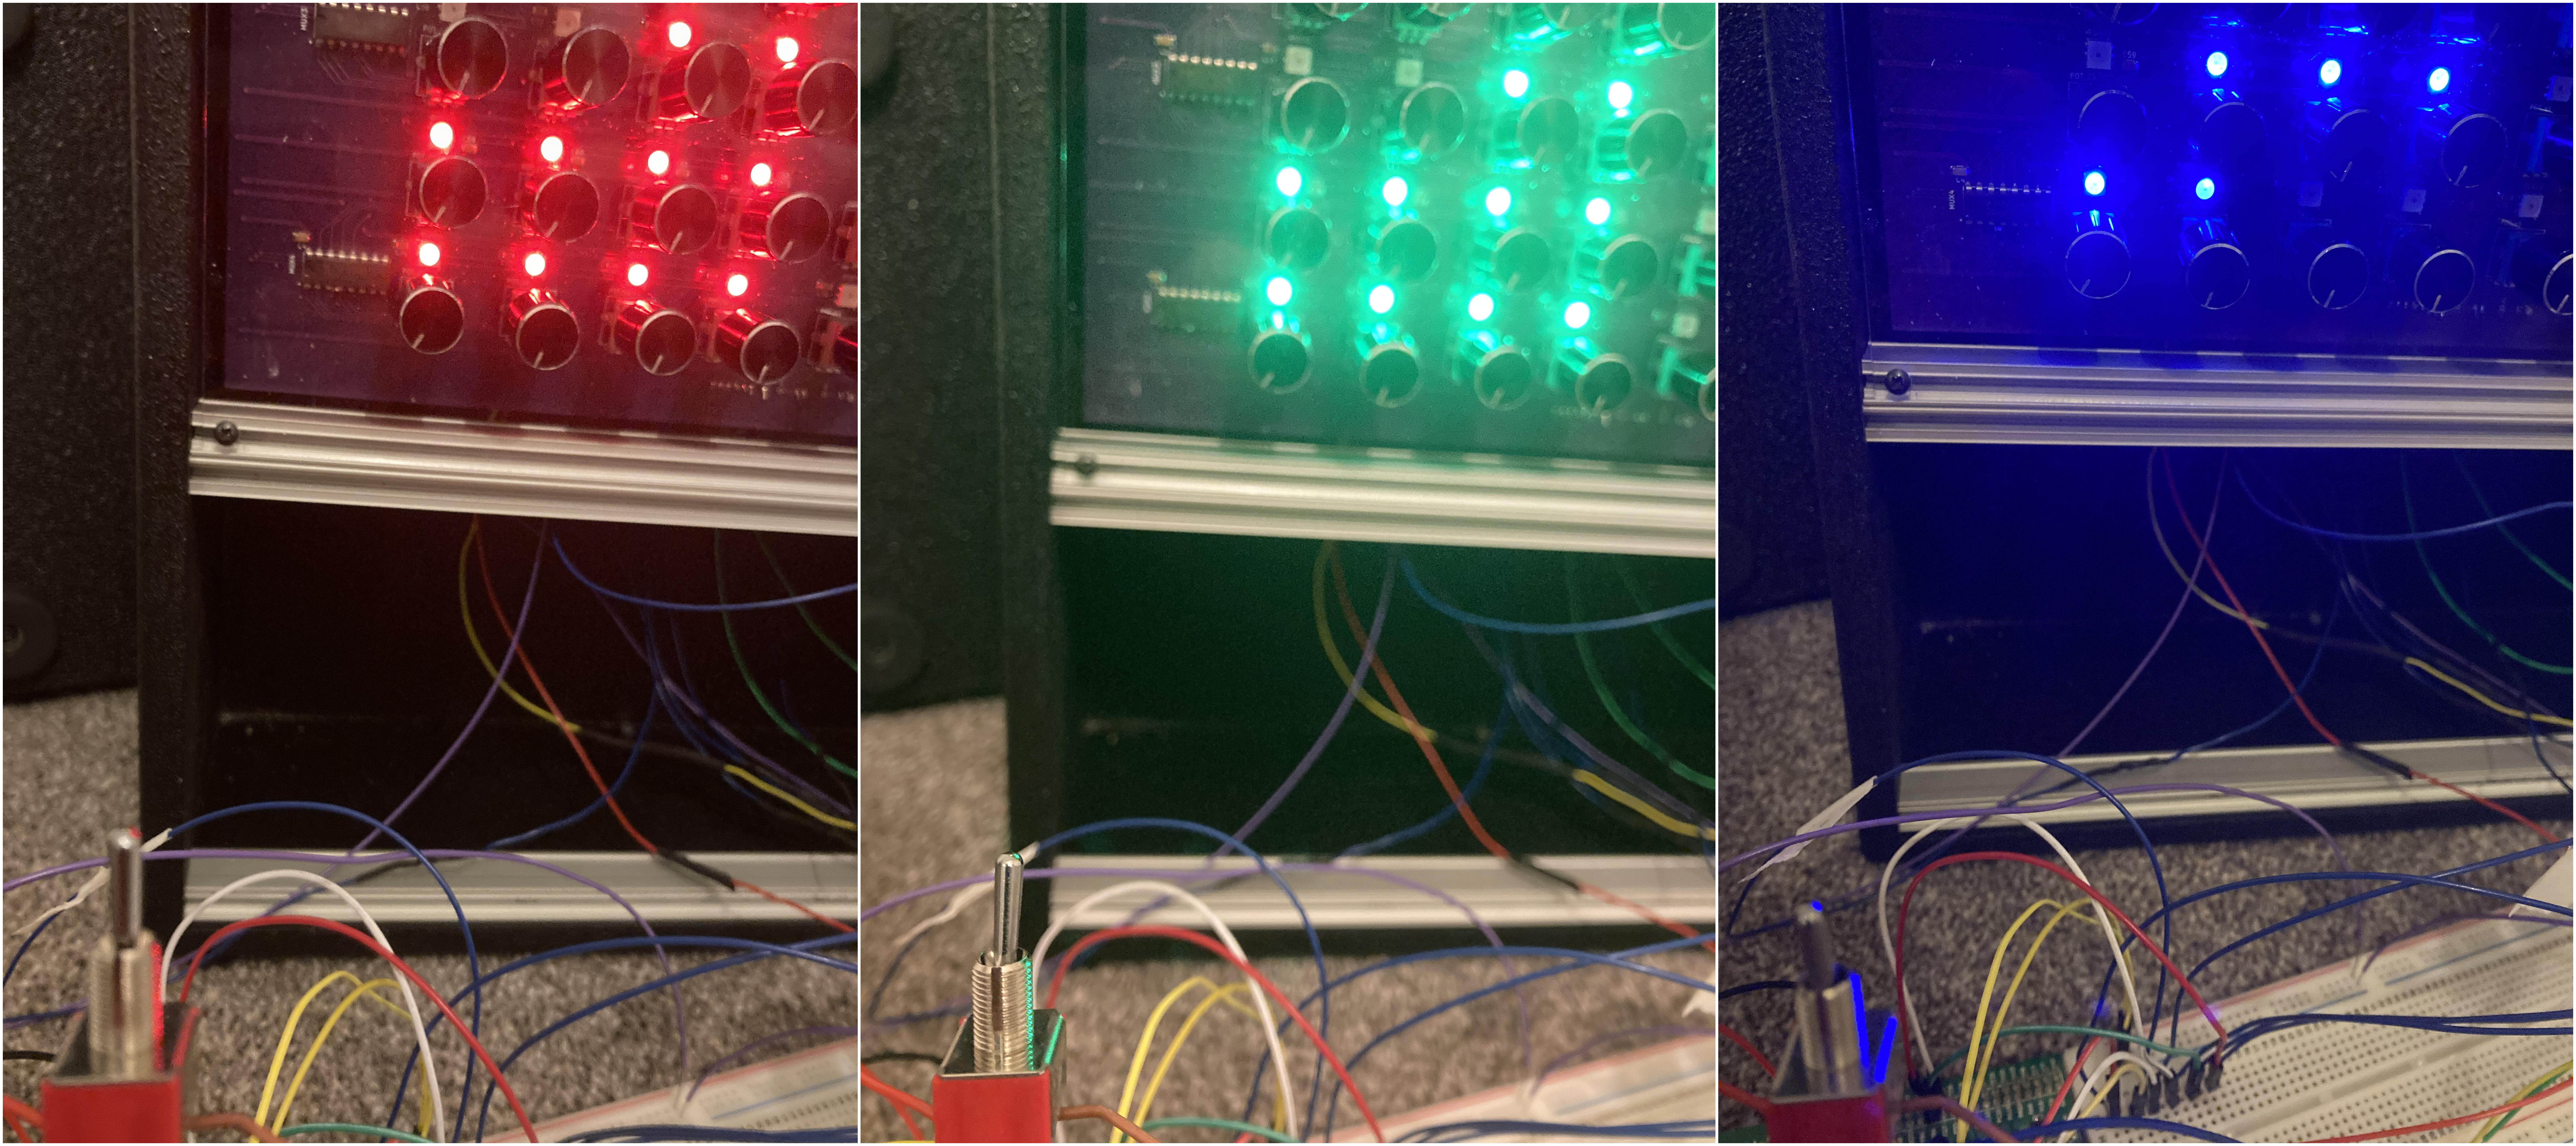
\includegraphics[width=0.9 \textwidth]{SPDT_test.jpg}}
    \caption{Testing the SPDT as a three-way switch.}
    \label{fig:SPDT_test}
\end{figure}

\begin{figure}[H]
    \centering
    \fbox{\includegraphics[width=0.95 \textwidth]{SPDT_code.jpg}}
    \caption{Source code for enabling three-way switching with a SPDT ON-OFF-ON switch.}
    \label{fig:SPDT_code}
\end{figure}

\begin{figure}[H]
    \centering
    \fbox{\includegraphics[width=0.9 \textwidth]{DPDT_to_SPDT.png}}
    \caption{DPDT ON-ON-ON configured as SPDT ON-OFF-ON.}
    \label{fig:DPDT_to_SPDT}
\end{figure}

\newpage

\subsection{User Interface}

The user-interface design of the sequencer's top and bottom front panels has been refined to enhance interaction and comfort. The top panel, illustrated in \autoref{fig:top_panel1}, is designed with clearly marked x and y axes to delineate four distinct quadrants. Around each potentiometer, white-dotted markings clearly define the minimum and maximum values, enhancing usability. The knobs are chosen for their lined markings, which allow users to easily see the current settings. Sufficient space between each potentiometer and LED ensures that users can comfortably adjust the knobs and clearly view the selected node.

\begin{figure}[H]
    \centering
    \fbox{\includegraphics[width=0.89 \textwidth]{top_panel.pdf}}
    \caption{Top panel design.}
    \label{fig:top_panel1}
\end{figure}
\newpage
The bottom panel is presented in \autoref{fig:bottom_panel1}. Each functional category – such as GLOBAL, CLOCK ENGINE, and TRIGGERS – is labelled. Rotary encoders, unlike potentiometers, are equipped with unmarked knobs to prevent confusion since the knob's position does not correlate with the displayed values on the seven-segment display. Strategically placed white dots between peripherals clarify their relationships. In the GATE MIXER module, arithmetic symbols are used to demonstrate gate addition, with colour-coded LEDs that indicate the active gate corresponding to each mode. Lastly, three-way switches are strategically positioned to facilitate the selection of clock divisions and the configuration of modes.

\begin{figure}[H]
    \centering
    \fbox{\includegraphics[width=0.95 \textwidth]{bottom_panel.pdf}}
    \caption{Bottom panel design.}
    \label{fig:bottom_panel1}
\end{figure}
\newpage

\section{Output}

With the sensor-reading system implemented and LED indicators integrated, the main task now is to enable the sequencer's output for controlling third-party synthesisers. The first step requires connecting the LED indicators to the potentiometers. This ensures that when a specific LED is lit, the system outputs the reading from the associated potentiometer. The second step involves enabling CV/gate functionality for direct integration with analogue synthesisers. The final step incorporates MIDI functionality, broadening compatibility with a wide range of third-party synthesisers.

\subsection{Sensor-Indicator Integration}


To prepare for future output capabilities,  the sensor reading from the potentiometer must correspond with the LED positioned directly above it. During the PCB design process, potentiometers were wired to the MUXs according to the software-centric pattern of the node transition algorithms. This ensured that the index of the ADC reading array would automatically match the currently lit LED position. Consequently, the adapted enum LedName, presented in \autoref{fig:mapping}, directly corresponds to the sensor readings without the need for additional mapping\footnote{As discussed in the \hyperref[wiring]{Wiring} section, this should not have been the case since whenever feasible, hardware-centric wiring should be prioritised.}. Thus, all that is required to fetch the desired potentiometer reading is to insert the enum global variable, current\_led\_position (of the LedName enum), as the index of the adc\_raw\_data array, which stores all of the readings of the potentiometers.

\subsection{CV/gate Functionality}

For the CV functionality of the sequencer, the binary data from the potentiometers must be converted to DC voltage values. The MCU features an integrated Digital-to-Analog Converter (DAC) that is used for this purpose. To set up the DAC, an MCU output pin is configured to analogue mode, and the DAC peripheral is enabled. A Timer peripheral is employed to schedule the DAC updates at a consistent rate, ensuring smooth CV output.

Initially, using DMA to automate the transfer of potentiometer readings from memory to the DAC was considered. However, in this application, the selection of which potentiometer reading to output is determined via user input, which alters the index of the data dynamically. This unpredictability in the index of the sensor data makes DMA less suitable, as DMA would require reconfiguration for each change in the sensor index, negating its benefits of reducing CPU load.
Given this scenario, employing interrupts is the most sensible strategy. The MCU is set up to use an ISR that triggers each time the Timer overflows. Within this ISR, the DAC's data holding register (DHR) is updated directly with the selected potentiometer's binary reading. 

To implement the gate functionality of the sequencer, an MCU Timer peripheral is configured to generate one-time pulses using its one-pulse mode \cite{STM32_reference}. This approach uses the Timer’s pulse-width modulation (PWM) capabilities to accurately set the pulse width. Once a pulse is generated, the Timer stops until it is manually retriggered, ensuring controlled timing of gate signals without continuous CPU involvement. The source code for implementing the CV/gate setup is detailed in \autoref{fig:CV_code} and confirmation of its operational success is documented in \autoref{fig:CV_test}\footnote{A change in the brightness of the green LED was observed when adjusting the potentiometer values, while the red LED blinked to signify each node transition.}.


\begin{figure}[H]
    \centering
    \fbox{\includegraphics[width=0.9 \textwidth]{CV_code.png}}
    \caption{Source code for CV/gate driver.}
    \label{fig:CV_code}
\end{figure}

\begin{figure}[H]
    \centering
    \fbox{\includegraphics[width=0.8 \textwidth]{CV_test.jpg}}
    \caption{Testing the CV/gate driver.}
    \label{fig:CV_test}
\end{figure}

\subsection{MIDI Functionality}

To implement MIDI functionality within the sequencer, the MCU uses its Universal Asynchronous Receiver-Transmitter (UART) capability to manage MIDI communications effectively. The setup includes configuring UART2 for MIDI output, setting an MCU output pin to alternate function mode, and enabling the UART peripheral. The baud rate is set precisely at 31,250 bits per second, aligning with MIDI standards to ensure consistent and reliable data transfers \cite{MIDI_protocol}. To improve efficiency, DMA is employed to transfer MIDI messages directly from memory to the UART peripheral\footnote{The only conceptual difference between this system and the system in \autoref{fig:spi} is that the SPI peripheral is replaced by the UART peripheral.}.

MIDI messages are structured to include a byte each for the command and channel, note number, and velocity value \cite{MIDI_protocol}. In this sequencer setup, messages are generated based on the user-programmed sequence and system timing logic. The potentiometer readings are converted into MIDI note values through a binary-to-MIDI note conversion function. The source code for implementing MIDI functionality is outlined in \autoref{fig:MIDI_code}.

\begin{figure}[H]
    \centering
    \fbox{\includegraphics[width=0.95 \textwidth]{MIDI_code.png}}
    \caption{Source code for MIDI driver.}
    \label{fig:MIDI_code}
\end{figure}

To test the driver, a DIN connector was sourced from the University labs. It was configured as specified in \autoref{fig:DIN}, using only a pair of \SI{220}{\ohm} resistors, since the other components are optional. When tested with the Behringer MS-1, the driver successfully transmitted MIDI messages, as evidenced in \autoref{fig:MIDI_test}.

\begin{figure}[H]
    \centering
    \fbox{\includegraphics[width=0.75 \textwidth]{DIN.png}}
    \caption{MIDI output wiring using a DIN connector (taken from \cite{MIDI_out}).}
    \label{fig:DIN}
\end{figure}

\begin{figure}[H]
    \centering
    \fbox{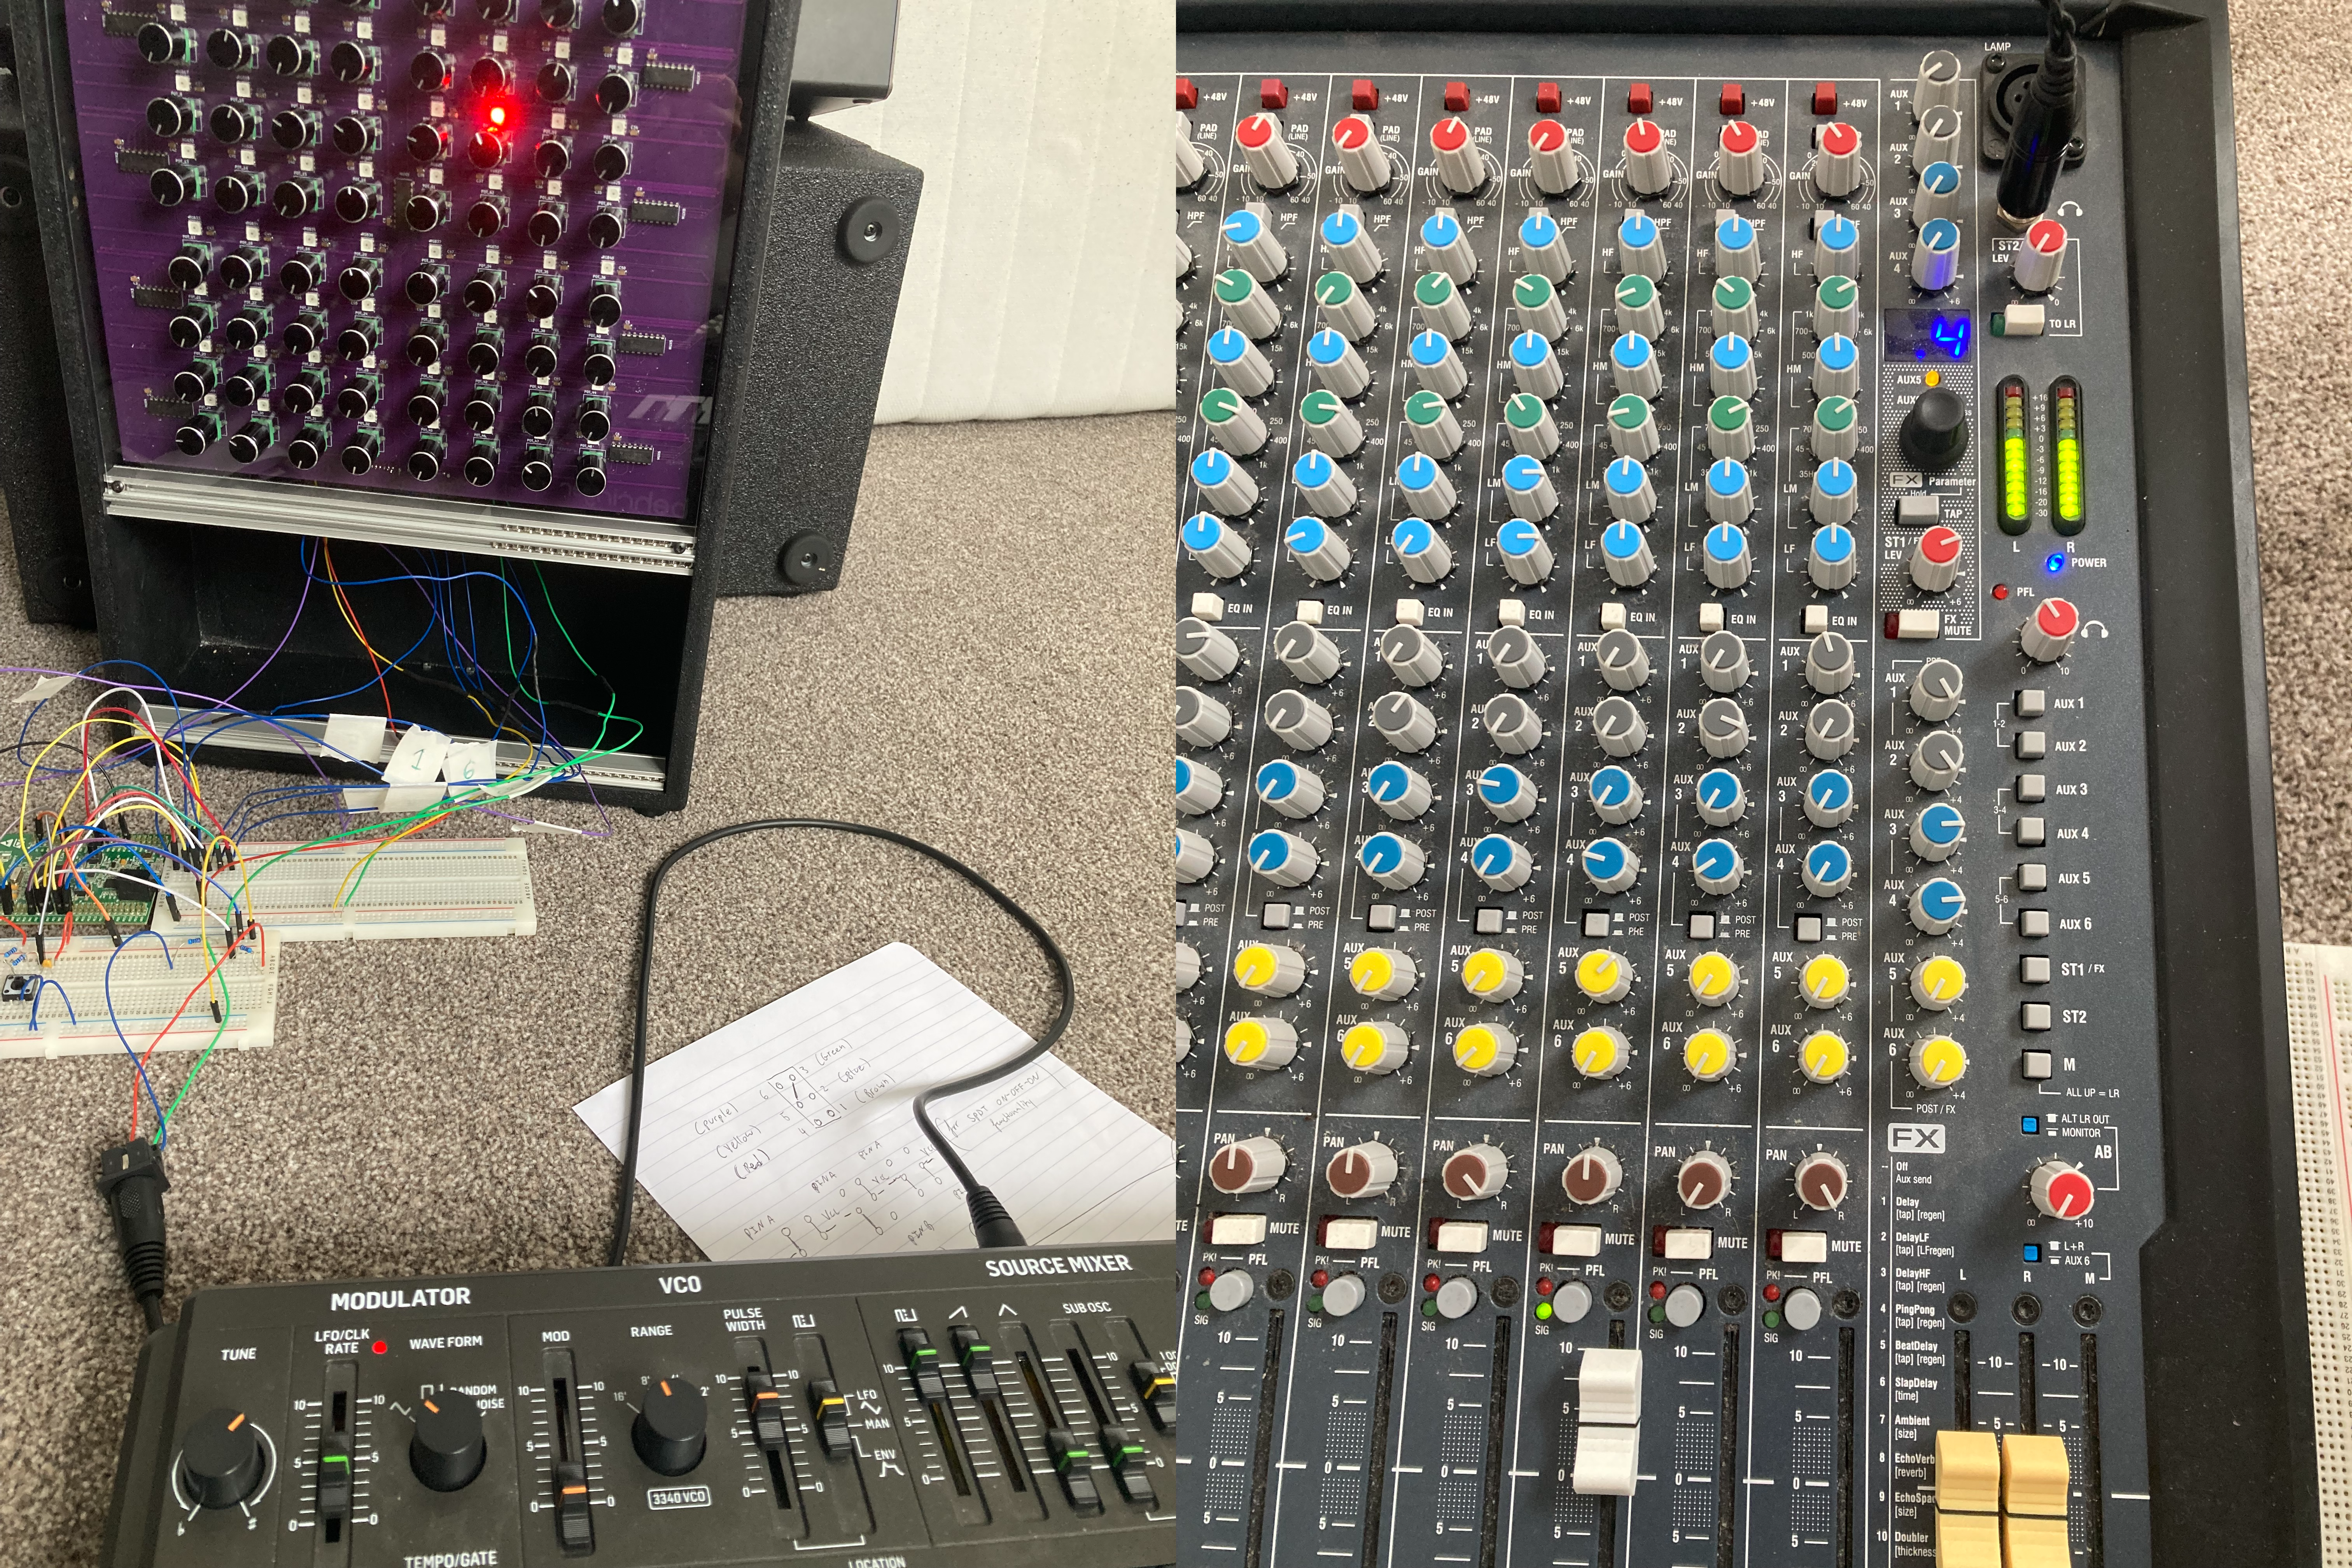
\includegraphics[width=0.75 \textwidth]{MIDI_test.png}}
    \caption{Testing the MIDI driver.}
    \label{fig:MIDI_test}
\end{figure}

\newpage

\section{Feedback}

In this section, feedback from users experienced with electronic devices is collected through surveys. Since only a component of the sequencer (the Complex Plane) is finalised and not the entire prototype (Ten\begin{CJK}{UTF8}{min}(天)\end{CJK}), comparing it to released products is premature. Instead, an evaluation of the Complex Plane is conducted to determine if refinements are needed before designing the recurring decimal algorithm. To enhance the evaluation, rhythmic presets were programmed to simulate basic patterns that could be generated by the recurring decimal algorithm engine.

Fifteen candidates participated in the survey presented in the \hyperref[appendix:survey]{User Survey} section of the appendix. The overall feedback was very positive. The vast majority agreed or strongly agreed that the device is easy to use, useful for both live performance and music composition, and innovative. Most users either agreed or remained neutral on whether the pitch range of the potentiometers was sufficient and if the product had commercial potential.

The most common qualitative feedback was that the sequencer is ergonomically easy to use and aesthetically pleasing. However, users suggested clarifying the role of the complex operator (perhaps by displaying an arrow from the origin to the selected node) and adding the ability to store presets of knob positions for live performances.






\newpage


\section{Project Management}

This section presents the development process of the sequencer, including initial planning, setbacks and adaptations encountered, and sustainability considerations.

\subsection{Initial Plan}

The development of the music sequencer was initially planned to be completed within a strict timeline, as detailed in \autoref{fig:gantt}. The project was divided into several key phases: core development, system integration and testing, and project documentation and evaluation.

The core development phase aimed to establish the software and hardware base required for the prototype. This included embedded programming and hardware design and assembly for both the Complex Plane and the recurring decimal algorithm engine. For embedded programming, the SPI and ADC drivers were necessary for the display interface and potentiometer input reading of the Complex Plane respectively. Timer drivers and rotary encoder integration with seven segment displays were important for the management of timing mechanisms and input processing for the recurring decimal algorithm engine. For hardware design and assembly, the Bill of Materials (BOM) development and components ordering were key steps for component identification and procurement. Additionally, the PCB designs, followed by the initial assembly, formed the basis of the physical structure of the prototype.

The system integration and testing phase was designed to ensure the integration of software and hardware and evaluate the combined system. It involved final testing and calibration to assess system performance and make adjustments for optimal functionality.

The project documentation and evaluation phase focused on documenting the development process and collecting user feedback for future development. This included project documentation to record the development process, system design, and testing results. User evaluation was also planned to gather feedback on the prototype's functionality and user experience for future improvements.

\begin{figure}[ht]
    \centering
    \fbox{\includegraphics[width=0.7 \textwidth]{Gantt.png}}
    \caption{Initial Gantt chart.}
    \label{fig:gantt}
\end{figure}

\subsection{Setbacks and Adaptation}

The initial timeline underestimated the time required to design the PCB for the Complex Plane. This was primarily due to the challenging task of figuring out how to design the PCB and manage wiring issues. As it was the designer's first PCB design, it was assumed that the software used (KiCad) would include an autorouting feature. However, it did not, necessitating manual routing. This manual process was time-consuming and took a week longer than anticipated. This miscalculation highlighted the need for more realistic time estimates and buffer periods in project planning, especially when using unfamiliar tools.

Another significant challenge was the delayed delivery of the PCB for the bottom panel, which contains the heart of the recurring decimal algorithm engine. The PCB arrived more than a week later than expected, which further pushed the project timeline back by two weeks. This delay emphasised the importance of having contingency plans and risk mitigation strategies in place.

Given the two-week delay caused by the extended PCB design time for the first PCB and late delivery of the second PCB, it became clear that completing both the Complex Plane and the recurring decimal algorithm engine within the remaining time was not feasible. As a result, a strategic decision was made to focus solely on the development of the Complex Plane. This decision was based on the assessment that completing one component to a high standard was preferable to delivering two incomplete or substandard components. The updated timeline reflecting these adjustments is detailed in \autoref{fig:gantt2}.



\begin{figure}[H]
    \centering
    \fbox{\includegraphics[width=0.7 \textwidth]{Gantt2.png}}
    \caption{Updated Gantt chart.}
    \label{fig:gantt2}
\end{figure}


\subsection{Sustainability Considerations}


Sustainability considerations were inherent to all stages of the sequencer's lifecycle.

The chassis is planned to be made of aluminium due to its high recyclability and low carbon footprint. Aluminium maintains its quality through multiple recycling processes, using only 5\% of the energy required for primary production \cite{ALUM}. Although there are financial concerns, aluminium aligns well with the sustainability policy.

The sequencer uses the Arm\textsuperscript{\textregistered} STM32F407VG MCU. STMicroelectronics ensures responsible and ethical sourcing, complying with the RMAP standard \cite{STM2}. Their commitment to sustainability is reflected in their strategy, ensuring the MCU comes from a traceable and sustainable supply chain \cite{STM3}.

The PCBs will be made from FR4 material, known for its durability and compliance with RoHS (Restriction of Hazardous Substances) standards, ensuring the product is free from harmful substances. The sequencer also avoids using rare components, making it easy to repair and minimising environmental impact.






\newpage
\section{Further Work}

This section outlines the future work required to complete the prototype, focusing on two main areas: enhancing features and reducing costs.

First, implementing the recurring decimal algorithm is essential for enabling rhythm generation, which drives the Complex Plane. This will involve designing the algorithm, controlling it with rotary encoders, and displaying it with seven-segment displays. Additionally, although CV/gate functionality is already implemented, quantisation of the CV output remains to be developed. This step is currently premature as it is necessary to first incorporate a bipolar power supply into the circuitry to communicate effectively with \(\pm 12V\) and \(\pm 15V\) analogue synthesiser systems. Once this is achieved, quantisation can be applied. In response to user feedback, implementing memory capabilities will be a valuable addition. This will enable the storage of user presets and enhance the overall functionality of the sequencer.

To reduce costs, the Summing Amplifier configuration, which has already been analysed and proven to be a cheaper alternative, will be implemented in the next development cycle. Furthermore, integrating a cheaper MCU directly into the PCB design, rather than using the discovery board, will enhance the professional quality of the final product and reduce costs. However, this integration should follow the development of the recurring decimal engine, as the discovery board is more suitable for prototyping purposes. Lastly, testing cheaper, more power-efficient, asynchronous RGB addressable LEDs to determine if their response time is sufficient will be crucial. If successful, this could further reduce costs without compromising performance.



\newpage
\section{Conclusion}
The development of the Complex Plane demonstrates significant advancements in user interaction and real-time performance capabilities. By integrating 64 potentiometers and RGB LEDs with the Arm\textsuperscript{\textregistered} STM32F407VG MCU, the project achieved precise sensor readings and intuitive visual feedback. The MUX topology and the SK9822 were selected for their reliability, and custom algorithms were successfully implemented to manage node transitions.

User feedback indicates high satisfaction with the Complex Plane's usability and innovation, though some suggestions for improvement were noted. The project also adhered to ethical standards, ensuring environmental sustainability and data privacy.

Future work will focus on implementing the recurring decimal algorithm to enable rhythm generation and integrating memory capabilities to store user presets. Additionally, cost reduction measures will include adopting the Summing Amplifier configuration, integrating a cheaper MCU directly into the PCB design, and testing more cost-effective asynchronous RGB addressable LEDs. These enhancements will further optimise the sequencer and broaden its application in both live performance and music composition.


\newpage



\bibliographystyle{ieeetr}
\bibliography{bib}

\newpage
\appendix

\section{Background}
\label{appendix:background}

This section begins with tracing the evolution of music sequencers from simple playback devices to complex, interactive tools for music creation and performance. It then highlights modern design features that meet user demands and examines how number theory underpins innovative sequencing techniques.

\subsection{Analysis of Music Sequencers}
\label{appendix:analysis}

The development of a new music sequencer requires an analysis of historical progression and contemporary trends within the music technology industry.

\subsubsection{Historical Analysis}

The origins of music sequencers date back to the late 18th century \cite{Bresin}. Early mechanical devices like the Music Box and the Weber Pianola Piano (see \autoref{fig:mechanical}) were functional music sequencers, but were non-interactive and could only play predetermined sequences \cite{Bresin}. The emergence of sequencers for live composition tools led to a transition from mechanically to electronically controlled models. This brought two key advantages: the control of music sequences in real-time and the decoupling of sequencers from fixed acoustic systems, making them versatile, general-purpose devices.

\begin{figure}[ht]
    \centering
    \fbox{\includegraphics[width=0.85 \textwidth]{mechanical.png}}
    \caption{The Music Box (a) and the Weber Pianola Piano (b) (taken from \cite{Bresin}).}
    \label{fig:mechanical}
\end{figure}

In the 1960s, Don Buchla and Bob Moog independently invented the first voltage-controlled sequencers \cite{Holmes}. These devices generated signals for pitch and rhythmic control, and enabled communication with various voltage-controlled systems. Typically, they featured manual triggering (e.g., the ability to transition to the next element of the sequence via a peripheral) and synchronisation to internal or external clocks, offering various sequence lengths across multiple channels \cite{Holmes}. Musicians expanded pattern variation by integrating multiple sequencers \cite{Strange}. This modular approach, wherein sequencers trigger one another, led to new forms of musical compositions and performances \cite{Strange}.

The analogue era, however, had its challenges. Synthesiser manufacturers employed inconsistent standards for sequencing parameters, varying in pitch control methods and pulse edge responses \cite{Kirk}. In response to these inconsistencies, a digital standard termed MIDI (Musical Instrument Digital Interface) emerged in the 1980s \cite{Diduck}. This standard enabled sequencers to act as standalone pattern generators, capable of creating various musical arrangements independently of connected devices.

The adoption of MIDI and the rapid expansion of digital memory capacity triggered a shift from voltage to digitally controlled sequencers, enabling sequence storage and novel sequencing methods \cite{Manning}. One noteworthy innovation was swing quantisation, a feature that allows musicians to fine-tune the groove of their sequences with digital precision \cite{Katz}. This functionality was incorporated into hardware samplers like the E-mu SP1200 from the late 1980s, contributing to the instrument's fame \cite{Milner}. As digital technology advanced, the integration of sequencers into personal computers introduced convenience and substantial changes in music production \cite{Huber}.

In the early 21st century, while there has been a broad shift towards user-centric design characterised by intuitive and tactile controls \cite{Moggridge}, the development of music sequencers has taken a more focused turn towards restraint in functionality \cite{Bjorn1}. 
This trend focuses on interfaces that offer key functionality without overwhelming users with excessive features. Accordingly, the current trend is towards balancing technological advancement with the practical needs and tactile ergonomics of users.

\subsubsection{Contemporary Analysis}

A contemporary analysis of music sequencers focuses on characteristics that have led to the success of specific products. This analysis introduces aspects of two sequencers: René by Make Noise and the Turing Machine by Music Thing Modular, highlighting their relevance in the music technology industry.

\subsubsubsection{René by Make Noise}

Make Noise's René features two distinct clock sources, termed `X-clock' and `Y-clock', for `cartesian' sequencing control \cite{Bjorn2}. The X-clock manages sequencing along the x-axis, while the Y-clock does so along the y-axis, providing flexible sequencing options on a two-dimensional grid  \cite{Bjorn2}. \autoref{fig:rene} compares René's 4x4 grid to a traditional 16-step sequencer, illustrating how varying clock rates influence sequencing patterns. Tony Rolando, the founder of Make Noise, highlights that René's unique sequencing capabilities `allow for live improv composition, using an analog-style sequencing interface' \cite{Rolando1}.

\begin{figure}[ht]
    \centering
    \fbox{\includegraphics[width=0.8 \textwidth]{rene.png}}
    \caption{Contrasting a traditional (1D) with a cartesian (2D) sequencer.}
    \label{fig:rene}
\end{figure}

\subsubsubsection{The Turing Machine by Music Thing Modular}

The Turing Machine by Music Thing Modular introduces an element of controlled randomness in sequence generation \cite{Turing}. It operates using a shift register, where binary values are stochastically introduced, allowing the user to lock and loop a particular sequence, making the output predictable and repeatable if desired \cite{Turing}. This method of algorithmic sequence generation enables musicians to explore generative music techniques. 

The significance of the Turing Machine in novel sequencer design is its mix of randomness and control. It indicates a shift towards a more adaptive, responsive composition style, where interacting with the machine is a key part of the creative process \cite{Bjorn2}. The Turing Machine's focus on algorithmic pattern generation and manipulation paves the way for examining how mathematical principles can be applied in music sequencer development.

\subsection{Music Sequencers and Number Theory}

In music sequencers, a connection exists between their design principles and the domain of number theory. The Euclidean algorithm is introduced to reveal the synergy between number theory and rhythm\footnote{While algorithms can generate notes, this project will specifically explore their potential for rhythm generation.} \cite{Toussaint1}. Contemporary research topics in this field, such as `Perfectly Balanced' and `Well-formed' rhythms, further uncover the relationship between number theory and music sequencer development.

\subsubsection{Euclidean Rhythms}

Euclidean rhythms, based on algorithmic music theory, incorporate into music sequencers a synergy between music composition and number theory \cite{Toussaint1}. These rhythms are generated using the Euclidean algorithm, which evenly distributes a specified number of beats across a sequence, ensuring mathematical precision and computational efficiency with $\mathcal{O}(n)$ time complexity \cite{Toussaint2}. 

The Euclidean algorithm, traditionally used to compute the greatest common divisor (GCD) of two natural numbers \cite{Toussaint1}, finds application in rhythm generation by representing variables $m$ and $k$ as binary sequences \cite{Toussaint2}. For instance, let $m = 13$ and $k = 5$. Initially, a binary sequence is created with $k$ `1’s (5 in total) and $m - k$ `0’s (8 in total): 

\begin{center}
[\textbar1\textbar1\textbar1\textbar1\textbar1\textbar\: 
\textbar0\textbar0\textbar0\textbar0\textbar0\textbar0\textbar0\textbar0\textbar]
\end{center}

The algorithm then appends a `0’ to each `1’, resulting in:

\begin{center}
[\textbar1\underline{0}\textbar1\underline{0}\textbar1\underline{0}\textbar1\underline{0}\textbar1\underline{0}\textbar\: \textbar0\textbar0\textbar0\textbar]
\end{center}

Continuing this process, the remaining `0’s are appended to each `1\underline{0}’ pattern:

\begin{center}
[\textbar10\underline{0}\textbar10\underline{0}\textbar10\underline{0}\textbar\:\;\textbar10\textbar10\textbar]
\end{center}

At this stage, it becomes apparent that there are not enough `0’s remaining to append to each `1\underline{0}’, leaving two out of five `1\underline{0}’ patterns intact. The remaining ‘10’ patterns are then appended to the `10\underline{0}’ patterns:

\begin{center}
[\textbar100\underline{10}\textbar100\underline{10}\textbar\: \textbar100\textbar]
\end{center}

When the right hand side of the sequence contains a pattern that appears only once (`100'), it signifies that the binary sequence has achieved optimal balance \cite{Toussaint2}, as \autoref{fig:euclid} demonstrates. Every sequence is initiated at node `0', and progresses clockwise in uniform time intervals until cycling back to node `0'. The utility of this algorithm as a rhythm generator now becomes evident when interpreting the `1's (gray nodes) as onsets, the `0's (white nodes) as rests, and attributing the length of the pattern (number of nodes) to the duration of the repeating sequence.

Stoichea by Rebel Technology makes use of the Euclidean algorithm to facilitate the creation of intricate rhythmic patterns \cite{Stoicha}. Similarly, the T1 by Torso Electronics incorporates Euclidean rhythms and introduces a dynamic feature allowing users to shift patterns either left or right \cite{Torso}. These implementations highlight the flexibility and adaptability of Euclidean rhythms, marking a departure from traditional sequencing methods. 

\begin{figure}[H]
    \centering
    \fbox{\includegraphics[width=0.75 \textwidth]{euclid.png}}
    \caption{Cyclic graph illustration of the Euclidean algorithm.}
    \label{fig:euclid}
\end{figure}

\subsubsection{Perfectly Balanced and Well-formed Rhythms}

Within the field of contemporary rhythm analysis, the concepts of balance and evenness are delineated by the Discrete Fourier Transform (DFT) \cite{Milne}. These concepts are implemented in the ground-breaking sequencer, Xronomorph, designed by Dynamic Tonality \cite{Milne}. To fully grasp the technical meanings of balance and evenness, one must understand how the DFT relates to rhythmic patterns.

Consider a vector $x \in [0, 1)^K$, containing $K$ real-numbered time values representing rhythmic onsets \cite{Milne}. These values are normalised to the range $[0, 1)$, with the period set at 1 \cite{Milne}. The vector is arranged in ascending order, such that $x_{0} < x_{1} < \cdots < x_{K-1}$ \cite{Milne}. An illustrative example is the ‘isochronous’ rhythm in \autoref{fig:PB}, where $x = \left\{ 0/12, 3/12, 6/12, 9/12\right\}$. These elements are then mapped to the unit circle in the complex plane as $z[k] =  \exp\left(2\pi ix[k]\right) \in \mathbb{C}$, resulting in a complex vector $z \in \mathbb{C}^K$ \cite{Milne}. Each $z[k]$ has a unit magnitude, and its angle signifies its time location as a proportion of the period, with the period's angle being $2\pi$ \cite{Milne}. The $t$-th coefficient of the DFT of the rhythm vector, denoted as $\mathcal{F}\{z[t]\}$ is given by the expression \cite{Milne}: 
\begin{equation}
\mathcal{F}\{z[t]\} = \frac{1}{K} \sum_{k=0}^{K-1}z[k] \exp\left(-2\pi itk/K\right)
\end{equation}

It is from this generalised DFT equation that both balance and evenness can be mathematically derived.

The concept of balance is encapsulated in the equation \cite{Milne}:

\begin{equation}
\text{balance} = 1 - |\mathcal{F}\{z[0]\}|, \in [0, 1]
\end{equation}
where $\mathcal{F}\{z[0]\}$ represents the $0$th DFT coefficient \cite{Milne}:

\begin{equation}
\mathcal{F}\{z[0]\} = \frac{1}{K} \sum_{k=0}^{K-1}z[k] 
\end{equation}
Balance ‘measures the distance of the rhythm’s centre of gravity (mean position) from the centre of the circle’ \cite{Milne}. In other words, by viewing each onset position on the circle as a 2D vector, the mean position would represent the resultant of all of these vectors. A `perfectly balanced' rhythm is characterised by a balance value of 1, indicating an even and harmonious distribution of energy \cite{Milne}, or a zero distance from the centre of the circle once all onset vectors are added (see ‘Perfectly Balanced’ in \autoref{fig:PB}).

On the other hand, evenness is denoted by the equation \cite{Milne}:
\begin{equation}
\text{evenness} = |\mathcal{F}\{z[1]\}|, \in [0, 1]
\end{equation}
where $\mathcal{F}\{z[1]\}$ is the first DFT coefficient \cite{Milne}:
\begin{equation}
\mathcal{F}\{z[1]\} = \frac{1}{K} \sum_{k=0}^{K-1}z[k]  \exp\left(-2\pi ik/K\right)
\end{equation}
\newpage
Perfect evenness, reflected by an evenness value of 1, is associated with isochronous rhythms: those that exhibit a uniform and regular temporal structure (see ‘Isochronous’ in \autoref{fig:PB}) \cite{Toussaint1}. Thus, evenness measures how similar a rhythm is to an isochronous one. Well-formed rhythms materialise when the aspiration for maximum evenness takes precedence, while adhering to the constraint of allowing no more than two sizes of inter-onset-intervals (IOIs) (see ‘Well-formed’ in \autoref{fig:PB}) \cite{Milne}. This constraint helps identify well-formed rhythms that might or might not be perfectly balanced or isochronous \cite{Milne}.

\begin{figure}[ht]
    \centering
    \fbox{\includegraphics[width=0.7 \textwidth]{PB.pdf}}
    \caption{Cyclic graph illustration of isochronous, well-formed, and perfectly balanced rhythms.}
    \label{fig:PB}
\end{figure}


XronoMorph stands out as a pioneering sequencer due to its capacity to generate both perfectly balanced and well-formed rhythms \cite{Milne}. This capability highlights the potential of integrating mathematical properties with sequencing functionalities, offering musicians a source of inspiration for the creation of innovative rhythmic designs\footnote{Notably, these rhythmic patterns appear across various musical traditions, suggesting a perennial and universal nature \cite{Toussaint1}.}.
\newpage

\section{Concept}

The conceptualisation phase proposes the use of recurring decimal algorithms for generating rhythmic patterns and introduces a novel method for representing sequences and controlling pitch. It then examines how these methods can be integrated.

\subsection{Rhythm Generation via Recurring Decimals}
\label{appendix:recurringdecimals}
Although number theory can be used to create rhythmic sequences, modern music sequencers do not seem to utilise recurring decimals for this purpose. This gap highlights an opportunity for innovation in rhythm generation using recurring decimals.

Given an integer numerator $n$ and a denominator $d$, if $d$ is not divisible by 2, 5, or their multiples, an infinite cyclical pattern known as a recurring decimal emerges \cite{Dickson}. For instance, choosing $n$ as 1 and $d$ as 7 results in the recurring decimal $0.\dot{1}4285\dot{7}$ when computing $1/7$. Consequently, employing just two numbers -- one for the numerator and one for the denominator -- can generate a cyclical pattern, with its length altered by the divisor $d$ \cite{Dickson}. 

Employing recurring decimal patterns for rhythmic generation is not yet well-defined. Transforming such a pattern into a rhythmic one requires an additional parameter: a comparator. By taking the same sequence and adding a comparator threshold value of 4, for instance, any number in the pattern $>=4$ may be represented as an onset while any number $<4$ may be represented as a rest. Therefore, the pattern $\dot{1}4285\dot{7}$ with a threshold value of 4 will have the onset pattern of $\dot{0}1011\dot{1}$. \autoref{fig:RD} illustrates how variations in rhythmic generation result from changing the values of the comparator for the same pattern.
\newline



\begin{figure}[ht]
    \centering
    \fbox{\includegraphics[width=0.9 \textwidth]{RD.png}}
    \caption{Cyclic graph illustration of a recurring decimal pattern given different comparator values.}
    \label{fig:RD}
\end{figure}
\newpage



The correlation between the value of the divisor and the length of the recurring decimal pattern \cite{Dickson} presents potential for new types of rhythmic patterns. Understanding, for instance, that the length of the recurring decimal sequence cannot exceed the value of the denominator facilitates the prediction of sequence characteristics \cite{Dickson}. Additionally, certain divisor values produce cyclic numbers, which, when multiplied by integers up to $n-1$ (where $n$ is the divisor value), maintain the pattern's integrity but alter the sequence's order \cite{Gardner}. \autoref{fig:cyclic} exposes how changing the numerator in a fraction with a cyclic denominator, while maintaining a constant comparator value, preserves the pattern but shifts its starting point. This comprehension paves the way for a three-parameter system -- involving the divisor, the dividend, and the comparator -- to swiftly create rhythmic patterns.

\begin{figure}[ht]
    \centering
    \fbox{\includegraphics[width=0.94 \textwidth]{cyclic.png}}
    \caption{Cyclic graph illustration of a recurring decimal pattern given different dividend values.}
    \label{fig:cyclic}
\end{figure}

\subsection{Sequence Visualisation and Pitch Control via the Complex Plane}
\label{appendix:complexplane}

The incorporation of a 2D coordinate system in music sequencing creates opportunities to use operations similar to those in complex number theory. For example, multiplying a point in an xy-plot by the complex operator $i$ rotates the point 90 degrees counterclockwise, changing its coordinates but keeping its magnitude \cite{Riley}. This idea can be applied to sequencer design for complex musical sequence transformations. Building on René's 2D grid, controlled by X-clock and Y-clock signals, an additional `C-clock' could be introduced. This clock would apply a complex operator to rotate any 2D vector on the grid. Such a feature permits intricate pattern manipulation, offering a new sequencing approach.
\newpage

\autoref{fig:complex} showcases three sequence patterns from the interaction of X, Y, and C clocks. The leftmost pattern emerges with the C-clock at sixteenth-note intervals and the X-clock at quarter-note intervals, creating a pattern that stretches along the x-axis and rotates about the origin. The rightmost pattern, with the Y-clock at quarter-note intervals, extends along the y-axis and also rotates. In the bottom pattern, the X and Y clocks match at quarter-note intervals, and the C-clock at sixteenth-note intervals, producing a pattern that expands along both axes and rotates. 

The Complex Plane serves a dual purpose: it allows users to visualise the sequence's current location, and each node governs the pitch associated with its position. An 8x8 grid is a practical choice for a prototype, as it is large enough to effectively demonstrate the functionality of the complex operator while remaining ergonomically manageable.

\begin{figure}[H]
    \centering
    \fbox{\includegraphics[width=0.9 \textwidth]{complex.png}}
    \caption{Patterns on the Complex Plane.}
    \label{fig:complex}
\end{figure}

\subsection{System Architecture}

The next key consideration is the design of the sequencing mechanism. The proposed approach utilises a trio of independent, synchronised cells that operate on a previously described recurring decimal algorithm. Each cell outputs a clock signal that directly influences the Complex Plane. Gate patterns are sent when specific conditions are met within each cell's algorithmic engine, which evaluates these conditions every local clock cycle. The control voltage (CV) determines the note value of the current node on the Complex Plane\footnote {In a MIDI setup, the CV (note) information is fetched before outputting the Note\_ON and Note\_OFF commands, as it is not possible to separate note and gate values in MIDI.}. Synchronisation across all clock parameters via an internal master clock facilitates the application of clock division, thereby introducing additional layers of rhythmic complexity built upon the foundational recurring decimal patterns. The gate outputs from each cell are then managed by a gate mixer to optimise flexibility in the sequencer's rhythmic capabilities. \autoref{fig:system} showcases the current high-level system design of the sequencer.



\begin{figure}[ht]
    \centering
    \fbox{\includegraphics[width=0.77 \textwidth]{system.png}}
    \caption{System design.}
    \label{fig:system}
\end{figure}

\section{Strategy}

After discussing the conceptual framework, attention shifts to the implementation strategy. The rationale behind choosing the Arm\textsuperscript{\textregistered} STM32F407VG MCU is presented, along with an explanation of how it will interface with the rest of the system.

\subsection{Core Development}

 The sequencer is hardware-based but relies on algorithmic computation for its primary functions. Given that it outputs only CV, rhythmic pulses, and MIDI signals, choosing a MCU over an array of digital integrated circuits is essential for compactness and cost-effectiveness \cite{Barlett}. Moreover, the programmable nature of embedded systems makes it ideal for prototyping, as crucial parameters can be adjusted via software without committing to a fixed hardware design. The Arm\textsuperscript{\textregistered} STM32F407VG MCU has been chosen for this task, although lower-spec MCUs like the STM32G071RB with its Cortex\textsuperscript{\textregistered}-M0+ processor could also suffice \cite{Yiu}. The selection is influenced by the designer's prior familiarity with its architecture, which is expected to expedite the development process.

 Furthermore, STMicroelectronics demonstrates a commitment to responsibly sourcing materials for their products, a principle embedded in their long-term values \cite{STM1}. They have implemented stringent requirements, such as mandating that suppliers adhere to the RMAP standard \cite{STM2}. This is part of their screening process to determine compliance with their Responsible Minerals Sourcing programme \cite{STM2}. STMicroelectronics also emphasises the importance of integrating sustainability practices into their company strategy, stating that it is crucial for their people, business, and society at large \cite{STM3}. 

\subsection{Hardware Interfacing}
\label{appendix:hardwareinterfacing}

The hardware interfacing strategy highlights the integration of sensors, indicators, and other components with the Arm\textsuperscript{\textregistered} STM32F407VG MCU. It focuses on key functionalities like tempo control, parameter visibility, and pitch adjustment, aimed at enhancing system flexibility and performance metrics.

Integrating sensors and indicators is essential for managing and monitoring the master internal clock and clock dividers, facilitating real-time tempo adjustments via the MCU's Timer peripherals. This does not only enable the control over the tempo, but will also play a role in synchronising the three clock dividers with the master clock. Each divider is controlled by its own switch, linked to the MCU, allowing for adjustments to their respective Timer's `prescaler' (\texttt{PSC}) register. 
\newpage
The X, Y, and C clock parameters are adjusted and displayed through rotary encoders and seven-segment displays, respectively. More specifically, these controls and displays are responsible for indicating the numerator, denominator, and threshold values for each clock, ensuring precise manipulation and monitoring. Additionally, each clock associated with the recurring decimal algorithm features a dedicated gate output and a summing gate mixer, facilitating the creation of complex rhythmic patterns (see \autoref{fig:bottom_panel}).

The Complex Plane, consisting of 64 analogue potentiometers and 64 RGB addressable LEDs, enables manual pitch adjustment for each node and provides visual feedback on the sequence's current position and mode\footnote{The mode determines the specific clock that will be displayed and managed by the peripherals. Upon selecting a mode, a corresponding colour representing the chosen clock will appear on the Complex Plane.} (see \autoref{fig:top_panel}). The LEDs interface with the MCU via SPI for a fast and reliable connection, while potentiometer readings are captured through a nine 8:1 MUX setup. This ensures rapid updating of each node's voltage value for precise and dynamic pitch control.

\begin{figure}[H]
    \centering
    \fbox{\includegraphics[width=0.7 \textwidth]{top_panel.pdf}}
    \caption{Top panel design.}
    \label{fig:top_panel}
\end{figure}

\begin{figure}[H]
    \centering
    \fbox{\includegraphics[width=0.89 \textwidth]{bottom_panel.pdf}}
    \caption{Bottom panel design.}
    \label{fig:bottom_panel}
\end{figure}


\newpage

\section{User Survey}
\label{appendix:survey}

Your privacy and the security of personal data are prioritised. Information collected through this questionnaire is processed lawfully, fairly, and transparently, used only for research purposes, and maintained in strict confidentiality. Data are stored securely and accessed only by the researcher conducting this study. Participation in this survey is entirely voluntary, and all responses are anonymised to ensure that individual participants cannot be identified. Participants have the right to access, rectify, or erase their data upon request. For any concerns regarding data handling, please contact ag1676@york.ac.uk.
\begin{enumerate}
\item To what extent do you think that the sequencer is easy to use? \\
% what is the difference between clearness, accuracy, completeness - Mohammad we have to be clear what these three words imply. A person doing this survey might be confused
% use the word 'improve' instead of 'increase'
O Strongly disagree O Disagree O Neither agree nor disagree O Agree O Strongly agree
\item To what extent do you think that the sequencer could be useful for live performances? \\
% To what extent do you think that the proposed user segment provides unambiquous requirements in this project?
O Strongly disagree O Disagree O Neither agree nor disagree O Agree O Strongly agree
\item To what extent do you think that the sequencer could be useful for composition? \\
%To what extent d you think that the proposed user segment improves the accuracy and correctness of of requirements in this project?
O Strongly disagree O Disagree O Neither agree nor disagree O Agree O Strongly agree
\item To what extent do you think that the pitch range of the sequencer is sufficiently wide?\\  
% change the word increase
O Strongly disagree O Disagree O Neither agree nor disagree O Agree O Strongly agree

\item To what extent do you think this sequencer is innovative? \\  O Strongly disagree O Disagree O Neither agree nor disagree O Agree O Strongly agree  

\item To what extent do you think this sequencer has potential for commercialisation? \\ 
O Strongly disagree O Disagree O Neither agree nor disagree O Agree O Strongly agree  

\newpage

In your opinion, what is the best feature of this sequencer?
% If no, can you please explain why not? 

...............................................................................................................\\
...............................................................................................................\\
...............................................................................................................\\
...............................................................................................................\\
...............................................................................................................\\
...............................................................................................................\\
...............................................................................................................\\
...............................................................................................................\\
...............................................................................................................\\
...............................................................................................................\\
...............................................................................................................\\
...............................................................................................................\\
...............................................................................................................\\
...............................................................................................................\\
...............................................................................................................\\
...............................................................................................................\\





In your opinion, what is a missing feature of this sequencer?
% If no, can you please explain why not? 

...............................................................................................................\\
...............................................................................................................\\
...............................................................................................................\\
...............................................................................................................\\
...............................................................................................................\\
...............................................................................................................\\
...............................................................................................................\\
...............................................................................................................\\
...............................................................................................................\\
...............................................................................................................\\
...............................................................................................................\\
...............................................................................................................\\
...............................................................................................................\\
...............................................................................................................\\
...............................................................................................................\\
...............................................................................................................\\
\end{enumerate}
\newpage

\section{PCB}
\subsection{Top Panel PCB}
\begin{figure}[H]
    \centering
    \fbox{\includegraphics[width=0.95 \textwidth]{TOP_PCB_SCHEMATIC.png}}
\end{figure}

\begin{figure}[H]
    \centering
    \fbox{\includegraphics[width=0.95 \textwidth]{TOP_PCB_TRACE.png}}
\end{figure}
\newpage


\subsection{Bottom Panel PCB}

\begin{figure}[H]
    \centering
    \fbox{\includegraphics[width=0.95 \textwidth]{BOTTOM_PCB_SENSORS.png}}
\end{figure}
\begin{figure}[H]
    \centering
    \fbox{\includegraphics[width=0.95 \textwidth]{BOTTOM_PCB_IO.png}}
\end{figure}
\begin{figure}[H]
    \centering
    \fbox{\includegraphics[width=0.95 \textwidth]{BOTTOM_PCB_TRACE.png}}
\end{figure}
\newpage















\section{Drivers}
\label{appendix:driverdevelopment}

\subsection{Multichannel Sensor Driver}

\begin{minted}{C}
#include "globals.h"
#include "systick.h"

void adc1_init(void) {
    
    /* Enable clock access to GPIOA */
    RCC->AHB1ENR |= RCC_AHB1ENR_GPIOAEN;
    
    /* Set PA1 to analogue mode */
    GPIOA->MODER |= (0x1UL << 2  | 0x1UL << 3);
    
    /* Enable clock access to ADC1 */
    RCC -> APB2ENR |= RCC_APB2ENR_ADC1EN;
    
    /* Configuire CR2 */
    ADC1->CR2 |= ADC_CR2_ADON;
    ADC1->CR2 |= ADC_CR2_DMA | ADC_CR2_DDS;
    
    /* Select external trigger on rising edge */
    ADC1 -> CR2 |= (1U<<28);
    ADC1 -> CR2 &= ~(1U<<29);
    
    /* Select Timer 2 TRGO event */
    ADC1 -> CR2 &= ~(1U<<24);
    ADC1 -> CR2 |= 1U<<25;
    ADC1 -> CR2 |= 1U<<26;
    ADC1 -> CR2 &= ~(1U<<27);
    
    /* Set sequence length (0) */
    ADC1->SQR1 = 0;
    
    /* No specified order */
    ADC1->SQR3 = 1;
}

void dma2_stream0_init(void) {

    /* Enable clock access to DMA */
    RCC -> AHB1ENR |=  RCC_AHB1ENR_DMA2EN;
    
    /* Disable DMA Stream */
    DMA2_Stream0 -> CR &= ~DMA_SxCR_EN;
    
    /* Wait till DMA is disabled */
    while((DMA2_Stream0->CR & DMA_SxCR_EN)){}
    
    /* Enable Circular mode */
    DMA2_Stream0->CR |= DMA_SxCR_CIRC;;
    
    /* Set memory transfer size to half-word*/
    DMA2_Stream0 -> CR |= (1U<<13);
    DMA2_Stream0 -> CR &= ~(1U<<14);
    
    /* Set peripheral transfer size to half-word */
    DMA2_Stream0 -> CR |= (1U<<11);
    DMA2_Stream0 -> CR &= ~(1U<<12);
    
    /* Enable memory address increment */
    DMA2_Stream0 -> CR |= DMA_SxCR_MINC;
    
    /* Set peripheral address */
    DMA2_Stream0->PAR = (uint32_t)(&(ADC1->DR));
    
    /* Set memory address */
    DMA2_Stream0-> M0AR = (uint32_t)(&adc_raw_data);
    
    /* Set number of transfer */
    DMA2_Stream0 -> NDTR = (uint16_t)TOTAL_CHANNELS;
    
    /* Enable transfer complete interrupt */
    DMA2_Stream0 -> CR |= DMA_SxCR_TCIE;
    
    /* Enable DMA Stream */
    DMA2_Stream0 -> CR |= DMA_SxCR_EN;
    
    /* Enable DMA interrupt in the NVIC */
    NVIC_EnableIRQ(DMA2_Stream0_IRQn);
}


void tim2_init(void) {

    /* Enable clock access to GPIOB */
    RCC->AHB1ENR |=  RCC_AHB1ENR_GPIOBEN;

    /* Configure GPIOB pins 0, 1, 2, 3, 4, 5 as outputs */
    GPIOB->MODER &= ~((0x3UL << (0 * 2)) | 
                      (0x3UL << (1 * 2)) | 
                      (0x3UL << (2 * 2)) |
                      (0x3UL << (3 * 2)) | 
                      (0x3UL << (4 * 2)) | 
                      (0x3UL << (5 * 2)));  

    GPIOB->MODER |=  ((0x1UL << (0 * 2)) | 
                      (0x1UL << (1 * 2)) | 
                      (0x1UL << (2 * 2)) |
                      (0x1UL << (3 * 2)) | 
                      (0x1UL << (4 * 2)) | 
                      (0x1UL << (5 * 2)));   

    /* Enable clock access */
    RCC->APB1ENR |= RCC_APB1ENR_TIM2EN;
    
    /* Set prescaler value */
    TIM2->PSC =  0; // 16Mhz / 1600 = 10k
    
    /* Set auto-reload value */
    TIM2->ARR = 1000 - 1; 

    /* Clear counter*/
    TIM2->CNT = 0;
    
    /* MMS (set to 'update') */
    TIM2->CR2 &= ~(1U<<4);
    TIM2->CR2 |= 1U<<5;
    TIM2->CR2 &= ~(1U<<6);
    
    /* Enable timer */
    TIM2->CR1 |= TIM_CR1_CEN;
    
    /* Enable TIM interrupt */
    TIM2->DIER |= TIM_DIER_UIE;
    
    /* Enable TIM interrupt in NVIC */
    NVIC_EnableIRQ(TIM2_IRQn);
}

void TIM2_IRQHandler(void) {   
    
    /* Check if update interrupt flag is set */
    if (TIM2->SR & TIM_SR_UIF) 
    { 
        /* Update channel index */
        current_channel++; 
        
        /* Wrap around at max channel number */
        current_channel %= TOTAL_CHANNELS; 
    
        /* Reset all relevant GPIOB pins before setting new value */
        GPIOB->BSRR = 0x3F << 16; 
    
         /* Set the bit corresponding to current_channel */
        GPIOB->BSRR = current_channel; 
    
        /* Clear update interrupt flag */
        TIM2->SR &= ~TIM_SR_UIF; 
    }
}

void DMA2_Stream0_IRQHandler(void) {

    /* Check if DMA transfer complete is set */
    if((DMA2 -> LISR) & DMA_LISR_TCIF0)
    {
        /* Clear the flag */
        DMA2 -> LIFCR |= DMA_LIFCR_CTCIF0;
    }
}
\end{minted}
\newpage
\subsection{SK9822 Driver}

\begin{minted}{C}
#include "globals.h"
#include "uart_dma.h"

#define PIN5_AF (1U<<11)
#define PIN6_AF (1U<<13)
#define PIN7_AF (1U<<15)
#define AFRL5_AF5 (1U<<22 | 1U<<20)
#define AFRL6_AF5 (1U<<26 | 1U<<24)
#define AFRL7_AF5 (1U<<30 | 1U<<28)
#define CR1_BR_DIV_8  (1U<<4)
#define DMA_SCR_DIR_M2P (1U<<6)
#define LED_COUNT    64

void spi1_dma_init(void) {

    /**************GPIO Configuration**************/
    
    /* Enable clock access to PORTA of SPI pins */
    RCC -> AHB1ENR |= RCC_AHB1ENR_GPIOAEN;

    /* Set SPI pins mode to alternate function mode */
    GPIOA -> MODER |= PIN5_AF;
    GPIOA -> MODER |= PIN7_AF;

    /* Set alternate type to AF5(SPI1) */
    GPIOA -> AFR[0] |= AFRL5_AF5;  // SCK
    GPIOA -> AFR[0] |= AFRL7_AF5;  // MOSI
    
    /**************SPI Configuration*****************/
    
    /* Enable clock access to SPI module */
    RCC -> APB2ENR |= RCC_APB2ENR_SPI1EN;

    /* Set clock divider : PCLK / 4 */
    SPI1 -> CR1 |= CR1_BR_DIV_8; 

    /* Set SPI to master mode */
    SPI1 -> CR1 |= SPI_CR1_MSTR;

    /* Set software slave management */
    SPI1 -> CR1 |= SPI_CR1_SSM;

    /* Set Internal slave select */
    SPI1 -> CR1 |= SPI_CR1_SSI;

    /* Set CPHA and CPOL */
    SPI1 -> CR1 |= SPI_CR1_CPOL | SPI_CR1_CPHA;

    /* Enable full-duplex */
    SPI1 -> CR1 &= ~(SPI_CR1_RXONLY);

    /* Set MSB first */
    SPI1 -> CR1 &= ~(SPI_CR1_LSBFIRST);

    /* Select to use DMA */
    SPI1 -> CR2 |= SPI_CR2_TXDMAEN;

    /* Enable SPI */
    SPI1 -> CR1 |= SPI_CR1_SPE;
}

void dma2_stream5_spi_tx_init(void) {
	
    /************DMA Configuration***********/
    
    /* Enable clock access to DMA */
    RCC -> AHB1ENR |= RCC_AHB1ENR_DMA2EN;
    
    /* Disable DMA stream */
    DMA2_Stream5 -> CR &= ~DMA_SxCR_EN;
    
    /* Wait till stream is disabled */
    while(DMA2_Stream5 -> CR & DMA_SxCR_EN){}
    
    /***** Configure DMA Stream parameters*****/
    
    /* Enable memory address increment */
    DMA2_Stream5 -> CR |= DMA_SxCR_MINC;
    
    /* Select channel 5 */
    DMA2_Stream5 -> CR |= (1U<<25 | 1U<<26);
    
    /* Set the transfer direction (Memory to Peripheral) */
    DMA2_Stream5 -> CR |=  DMA_SCR_DIR_M2P;
    
    /* Enable transfer complete interrupt */
    DMA2_Stream5 -> CR |= DMA_SxCR_TCIE;
    
    /* enable transfer error interrupt */
    DMA2_Stream5 -> CR |= DMA_SxCR_TEIE;
    
    /* Disable direct mode */
    DMA2_Stream5 -> FCR |= DMA_SxFCR_DMDIS;
    
    /* Set DMA FIFO threshold */
    DMA2_Stream5 -> FCR |= DMA_SxFCR_FTH_1 | DMA_SxFCR_FTH_0;
    
    /* Enable DMA interrupt in the NVIC */
    NVIC_EnableIRQ(DMA2_Stream5_IRQn);
}

void dma2_stream_spi_transfer(void) {
	
    /* Clear interrupt flags */
    DMA2 -> HIFCR = DMA_HIFCR_CTEIF5 | DMA_HIFCR_CTCIF5;
    
    /* Set the peripheral address */
    DMA2_Stream5 -> PAR = (uint32_t)(&(SPI1 -> DR));
    
    /* Set the memory address */
    DMA2_Stream5 -> M0AR = (uint32_t)led_buffer;
    
    /* Set memory length */
    DMA2_Stream5 -> NDTR = sizeof(led_buffer);
    
    /* Enable the DMA Stream */
    DMA2_Stream5 -> CR |= DMA_SxCR_EN;
}

void DMA2_Stream5_IRQHandler(void) {
	
    if((DMA2 -> HISR) & DMA_HISR_TCIF5)
    {
        for (int i = 0; i < FRAME_SIZE; i++)
                led_buffer[led_offsets[new_led_position] + i] = off[i];
        
        /* Clear the flag */
        DMA2 -> HIFCR |= DMA_HIFCR_CTCIF5;
    }
    else if ((DMA2 -> HISR) & DMA_HISR_TEIF5)
    {
        /* print error */
    
    
        /* Clear the flag */
        DMA2 -> HIFCR |= DMA_HIFCR_CTEIF5;
    }
}

\end{minted}
\newpage
\subsection{Push-buttons and Three-way Switch Driver}

\begin{minted}{C}
#include "globals.h"
#include "pulse_trig.h"
#include "systick.h"
#include "uart_dma.h"

void pd0_exti_init(void) {

    /* Disable global interrupt */
    __disable_irq();
    
    /* Enable clock access from GPIOD */
    RCC -> AHB1ENR |= RCC_AHB1ENR_GPIODEN;
    
    /* Enable clock access for SYSCFG */
    RCC -> APB2ENR |= RCC_APB2ENR_SYSCFGEN;
    
    /* Set PA0 as input pin */
    GPIOD -> MODER &= ~(1U<<0);
    GPIOD -> MODER &= ~(1U<<1);
    
    /* Set mode to pull-down */
    GPIOD->PUPDR |= (1UL << (0 * 2));
    
    /* Select PORTA for EXTI0 */
    SYSCFG -> EXTICR[0] |= SYSCFG_EXTICR1_EXTI0_PD;
    
    /* Unmask EXTI0 */
    EXTI -> IMR |= EXTI_IMR_MR0;
    
    /* Select falling edge trigger */
    EXTI -> FTSR |= EXTI_FTSR_TR0;
    
    /* Enable EXTI0 line in NVIC */
    NVIC_EnableIRQ(EXTI0_IRQn);
    
    /* Enable global interrupt */
    __enable_irq();
}

void EXTI0_IRQHandler(void) {
    if ((EXTI->PR & EXTI_PR_PR0) != 0) {

        uint32_t current_time = get_tick();

        /* Clear the interrupt pending bit */
        EXTI->PR |= EXTI_PR_PR0;  

        if (current_time - last_interrupt_time > 150)
        {
        	last_interrupt_time = current_time;
        	move_X();
        }
    }
}

void pd1_exti_init(void) {

    /* Disable global interrupt */
    __disable_irq();
    
    /* Enable clock access from GPIOA */
    RCC -> AHB1ENR |= RCC_AHB1ENR_GPIODEN;
    
    /* Enable clock access for SYSCFG */
    RCC -> APB2ENR |= RCC_APB2ENR_SYSCFGEN;
    
    /* Set PD1 as input pin */
    GPIOD -> MODER &= ~(1U<<2);
    GPIOD -> MODER &= ~(1U<<3);
    
    /* Set mode to pull-down */
    GPIOD->PUPDR |= (1UL << (1 * 2));
    
    /* Select PORTD for EXTI1 */
    SYSCFG->EXTICR[0] |= SYSCFG_EXTICR1_EXTI1_PD;
    
    /* Unmask EXTI1 */
    EXTI->IMR |= EXTI_IMR_MR1;
    
    /* Select falling edge trigger */
    EXTI->FTSR |= EXTI_FTSR_TR1;
    
    /* Enable EXTI1 line in NVIC */
    NVIC_EnableIRQ(EXTI1_IRQn);
    
    /* Enable global interrupt */
    __enable_irq();
}

void EXTI1_IRQHandler(void) {

    if ((EXTI->PR & EXTI_PR_PR1) != 0) {
    
        uint32_t current_time = get_tick();
    
        EXTI->PR |= EXTI_PR_PR1;
    
        if (current_time - last_interrupt_time > 150) {
    
            last_interrupt_time = current_time;
    
            move_Y();
        }
    }
}

void pd2_exti_init(void) {

    /* Disable global interrupt */
    __disable_irq();
    
    /* Enable clock access from GPIOA */
    RCC -> AHB1ENR |= RCC_AHB1ENR_GPIODEN;
    
    /* Enable clock access for SYSCFG */
    RCC -> APB2ENR |= RCC_APB2ENR_SYSCFGEN;
    
    /* Set PD2 as input pin */
    GPIOD -> MODER &= ~(1U<<4);
    GPIOD -> MODER &= ~(1U<<5);
    
    /* Set mode to pull-down */
    GPIOD->PUPDR |= (1UL << (2 * 2));
    
    /* Select PORTD for EXTI2 */
    SYSCFG->EXTICR[0] |= SYSCFG_EXTICR1_EXTI2_PD;
    
    /* Unmask EXTI2 */
    EXTI->IMR |= EXTI_IMR_MR2;
    
    /* Select falling edge trigger */
    EXTI->FTSR |= EXTI_FTSR_TR2;
    
    /* Enable EXTI2 line in NVIC */
    NVIC_EnableIRQ(EXTI2_IRQn);
    
    /* Enable global interrupt */
    __enable_irq();
}

void EXTI2_IRQHandler(void) {

    if (EXTI->PR & EXTI_PR_PR2) {
    
        uint32_t current_time = get_tick();
    
        EXTI->PR |= EXTI_PR_PR2;
    
        if (current_time - last_interrupt_time > 150) {
    
            last_interrupt_time = current_time;
    
            move_C();
    
        }
    }
}

void pe3_exti_init(void) 
{
    /* Disable global interrupt */
    __disable_irq();
    
    /* Enable clock access from GPIOE */
    RCC -> AHB1ENR |= RCC_AHB1ENR_GPIOEEN;
    
    /* Enable clock access for SYSCFG */
    RCC -> APB2ENR |= RCC_APB2ENR_SYSCFGEN;
    
    /* Set PE3 as input pin */
    GPIOE -> MODER &= ~(1U<<6);
    GPIOE -> MODER &= ~(1U<<7);
    
    /* Set PE3 to pull-down */
    GPIOE->PUPDR &= ~(1U<<6);
    GPIOE->PUPDR |=   1U<<7;
    
    /* Select PORTE for EXTI3 */
    SYSCFG->EXTICR[0] |= SYSCFG_EXTICR1_EXTI3_PE;
    
    /*Unmask EXTI3 */
    EXTI->IMR |= EXTI_IMR_MR3;
    
    /* Select rising edge trigger */
    EXTI->RTSR |= EXTI_RTSR_TR3;
    
    /* Select falling edge trigger */
    EXTI->FTSR |= EXTI_FTSR_TR3;
    
    /* Enable EXTI3 line in NVIC */
    NVIC_EnableIRQ(EXTI3_IRQn);
    
    /* Enable global interrupt */
    __enable_irq();
}

void EXTI3_IRQHandler(void) {

    if (EXTI->PR & EXTI_PR_PR3)
    {
        uint32_t current_time = get_tick();
    
        /* Clear PR flag*/
        EXTI->PR |= EXTI_PR_PR3;
    
        /* Apply debouncing */
        if (current_time - last_interrupt_time > 150)
        {
            last_interrupt_time = current_time;
    
            /* Read states of PE3 and PE4 */
            uint32_t pe3_state = (GPIOE->IDR & (1 << 3)) >> 3;
            uint32_t pe4_state = (GPIOE->IDR & (1 << 4)) >> 4;
            uint32_t state = (pe4_state << 1) | pe3_state;
    
            /* Handle the mode based on the state */
            switch(state)
            {
                case 0b00:
                    display_red_led();    // Both off
                    break;
                case 0b01:
                    display_green_led();  // PE3 on, PE4 off
                    break;
                case 0b10:
                    display_blue_led();   // PE3 off, PE4 on
                    break;
                default:
                    break;
            }
        }
    }
}

void pe4_exti_init(void) {
    
    /* Disable global interrupt */
    __disable_irq();
    
    /* Enable clock access from GPIOA */
    RCC -> AHB1ENR |= RCC_AHB1ENR_GPIOEEN;
    
    /* Enable clock access for SYSCFG */
    RCC -> APB2ENR |= RCC_APB2ENR_SYSCFGEN;
    
    /* Set PE4 as input pin */
    GPIOE -> MODER &= ~(1U<<8);
    GPIOE -> MODER &= ~(1U<<9);
    
    // Set mode to pull-down
    GPIOE->PUPDR &= ~(1U<<8);
    GPIOE->PUPDR |=  (1U<<9);
    
    /* Select PORTE for EXTI4 */
    SYSCFG->EXTICR[1] |= SYSCFG_EXTICR2_EXTI4_PE;
    
    /*Unmask EXTI4 */
    EXTI->IMR |= EXTI_IMR_MR4;
    
    /* Select rising edge trigger */
    EXTI->RTSR |= EXTI_RTSR_TR4;
    
    /* Select falling edge trigger */
    EXTI->FTSR |= EXTI_FTSR_TR4;
    
    /* Enable EXTI2 line in NVIC */
    NVIC_EnableIRQ(EXTI4_IRQn);
    
    /* Enable global interrupt */
    __enable_irq();
}

void EXTI4_IRQHandler(void) {

    if (EXTI->PR & EXTI_PR_PR4) {
    
        uint32_t current_time = get_tick();
    
        /* Clear PR flag*/
        EXTI->PR |= EXTI_PR_PR4;
    
        /* Apply debouncing */
        if (current_time - last_interrupt_time > 150)
        {
            last_interrupt_time = current_time;
    
            /* Read states of PE3 and PE4 */
            uint32_t pe3_state = (GPIOE->IDR & (1 << 3)) >> 3;
            uint32_t pe4_state = (GPIOE->IDR & (1 << 4)) >> 4;
            uint32_t state = (pe4_state << 1) | pe3_state;
    
            /* Handle the mode based on the state */
            switch(state)
            {
                case 0b00:
                    display_red_led();    // Both off
                    break;
                case 0b01:
                    display_green_led();  // PE3 on, PE4 off
                    break;
                case 0b10:
                    display_blue_led();   // PE3 off, PE4 on
                    break;
                default:
                    break;
            }
        }
    }
}
\end{minted}

\newpage
\subsection{CV/gate Driver}
\begin{minted}{C}
#include "globals.h"

void dac_init(void) {

    /* Enable clock for GPIOA */
    RCC -> AHB1ENR |= RCC_AHB1ENR_GPIOAEN;
    
    /* Set PA4 to analog mode (DAC_OUT1) */
    GPIOA -> MODER |= GPIO_MODER_MODER4;
    
    /* Enable DAC clock */
    RCC->APB1ENR |= RCC_APB1ENR_DACEN;
    
    /* Timer 6 is set by default as TRGO upon reset */
    
    /* Enable DAC channel 1 */
    DAC->CR |= DAC_CR_EN1;
}

void tim6_init(void) {

    /* Enable Timer6 clock */
    RCC->APB1ENR |= RCC_APB1ENR_TIM6EN;

    /* No prescaler */
    TIM6->PSC = 0;

    /* Auto-reload value */
    TIM6->ARR = 8399;

    /* Update event as trigger output (TRGO) */
    TIM6->CR2 |= TIM_CR2_MMS_1;

    /* Enable timer */
    TIM6->CR1 |= TIM_CR1_CEN;

    /* Enable TIM6 interrupt */
    TIM6->DIER |= TIM_DIER_UIE;

    /* Enable TIM interrupt in NVIC */
    NVIC_EnableIRQ(TIM6_DAC_IRQn);
}

void TIM6_DAC_IRQHandler(void) {

    if (TIM6->SR & TIM_SR_UIF)
    {
        /* Assign currently selected sensor to DAC */
        DAC->DHR12R1 = adc_raw_data[(int)current_led_position];
    
        /* Clear flag */
        TIM6->SR &= ~TIM_SR_UIF;
    }
}

void tim4_pb6_pulse_init(void) {

    /* Enable clock for TIM4 */
    RCC->APB1ENR |= RCC_APB1ENR_TIM4EN;

    /* No prescaler */
    TIM4->PSC = 0;

    /* Auto-reload value */
    TIM4->ARR = 999;

    /* Output goes low after clock cycles */
    TIM4->CCR1 = 500;

    /* Set channel 1 as output */
    TIM4->CCMR1 &= ~TIM_CCMR1_CC1S;

    /* Set to PWM1 mode */
    TIM4->CCMR1 |= TIM_CCMR1_OC1M_2 | TIM_CCMR1_OC1M_1;
    
    /* Enable compare mode for channel 1 */
    TIM4->CCER |= TIM_CCER_CC1E;

    /* Enable one-pulse mode */
    TIM4->CR1 |= TIM_CR1_OPM;

    /* Force update to apply the settings */
    TIM4->EGR = TIM_EGR_UG;
    
    /* Start the timer */
    TIM4->CR1 |= TIM_CR1_CEN;
    
    /* Enable clock for GPIO B */
    RCC->AHB1ENR |= RCC_AHB1ENR_GPIOBEN;
    
    /* Set GPIOB6 mode to alternate function */
    GPIOB->MODER |= GPIO_MODER_MODER6_1;
    
    /* Set alternate function to AF2 (TIM4) */
    GPIOB->AFR[0] |= GPIO_AFRL_AFSEL6_1;
}

void trigger_pulse(void) {

    /* Re-trigger the timer */
    TIM4 -> CR1 |= TIM_CR1_CEN;
}
\end{minted}
\newpage
\subsection{MIDI Driver}
\begin{minted}{c}

#include "globals.h"

#define CLK      16000000
#define UART_BAUDRATE 31250

void uart2_tx_init(void) {

    /* Enable Clock access to GPIOA */
    RCC -> AHB1ENR |= RCC_AHB1ENR_GPIOAEN;
    
    /* Set PA2 mode to alternate function mode */
    GPIOA -> MODER |=  GPIO_MODER_MODER2_1;
    
    /* Set PA2 alternate function type to AF7 (UART2) */
    GPIOA -> AFR[0] |= GPIO_AFRL_AFSEL2_0 | 
                           GPIO_AFRL_AFSEL2_1 |       
                           GPIO_AFRL_AFSEL2_2;
    
    /* Enable clock access to UART2 */
    RCC -> APB1ENR |= RCC_APB1ENR_USART2EN;
    
    /* Set baudrate */
    USART2 -> BRR = (uint16_t)((CLK + UART_BAUDRATE/2U) / UART_BAUDRATE);
    
    /* Select to use DMA for TX */
    USART2 -> CR3 = USART_CR3_DMAT;
    
    /* Set transfer direction */
    USART2 -> CR1 = USART_CR1_TE;
    
    /* Clear TC flag */
    USART2 -> SR &= ~(USART_SR_TC);
    
    /* Enable TC interrupt */
    USART2 -> CR1 |= USART_CR1_TCIE;
    
    /* Enable uart module */
    USART2 -> CR1 |= USART_CR1_UE;
    
    /* 1 stop bit */
    USART2 -> CR2 &= ~(USART_CR2_STOP);
}

void dma1_stream6_init(void) {

    /* Enable clock access to DMA1 */
    RCC -> AHB1ENR |= RCC_AHB1ENR_DMA1EN;
    
    /* Disable DMA Stream */
    DMA1_Stream6 -> CR &= ~(DMA_SxCR_EN);
    
    /* Wait until DMA is disabled */
    while((DMA1_Stream6 -> CR & DMA_SxCR_EN)){}
    
    /* Set peripheral address */
    DMA1_Stream6 -> PAR = (uint32_t) (&(USART2 -> DR));
    
    /* Select Channel 4 */
    DMA1_Stream6 -> CR &= ~(DMA_SxCR_CHSEL_0);
    DMA1_Stream6 -> CR &= ~(DMA_SxCR_CHSEL_1);
    DMA1_Stream6 -> CR |=   DMA_SxCR_CHSEL_2;
    
    /* Enable memory address increment */
    DMA1_Stream6 -> CR |= DMA_SxCR_MINC;
    
    /* Set transfer direction (memory to peripheral) */
    DMA1_Stream6 -> CR |=   DMA_SxCR_DIR_0;
    DMA1_Stream6 -> CR &= ~(DMA_SxCR_DIR_1);
    
    /* Set transfer complete interrupt */
    DMA1_Stream6 -> CR |= DMA_SxCR_TCIE;
    
    /* Enable DMA Stream6 Interrupt in NVIC */
    NVIC_EnableIRQ(DMA1_Stream6_IRQn);
}

void dma1_stream6_uart_tx(uint8_t * midi_message, uint32_t length) {
    
    /* Disable DMA Stream */
    DMA1_Stream6 -> CR &= ~(DMA_SxCR_EN);
    
    /* Set memory address */
    DMA1_Stream6 -> M0AR = (uint32_t)midi_message;
    
    /* Set number of transfers */
    DMA1_Stream6 -> NDTR = length;
    
    /* Enable DMA stream */
    DMA1_Stream6 -> CR |= DMA_SxCR_EN;
}

#define MIDI_NOTE_RANGE 36
#define POT_RESOLUTION 4095    // Assuming 16-bit resolution (0-65535)
#define MIDI_START_NOTE 36     // Starting MIDI note number (C3)

void MIDI_send(uint8_t channel, uint8_t command, uint8_t note, uint8_t velocity) {
	
    static uint8_t midi_buffer[3];
    
    /* MIDI command and channel number */
    midi_buffer[0] = command | (channel - 1);  
    midi_buffer[1] = note;
    midi_buffer[2] = velocity;
    
    /* Trigger DMA to send the MIDI message */
    dma1_stream6_uart_tx(midi_buffer, 3);
}




uint16_t map_to_midi(uint16_t pot_value) {

    /* Calculate MIDI note based on potentiometer reading */
    uint16_t midi_note = (pot_value * MIDI_NOTE_RANGE) / 
                         POT_RESOLUTION + MIDI_START_NOTE;
    return midi_note;
}

void DMA1_Stream6_IRQHandler(void) {

    if((DMA1 -> HISR) & DMA_HISR_TCIF6 ) {
    
        /* clear transfer complete flag */
        DMA1 -> HIFCR = DMA_HIFCR_CTCIF6; 
    }
}
\end{minted}
\newpage
\subsection{SysTick Driver}
\begin{minted}{c}

volatile uint32_t g_curr_tick;
volatile uint32_t g_curr_tick_p;

/* Initialise SysTick to count every ms */
void systick_init_millisecond(void) {
    
    /* Set reload register to 1ms */
    SysTick -> LOAD = (16000000 / 1000) - 1;
    
    /* Reset the SysTick counter value */
    SysTick -> VAL = 0;

    /* Enable SysTick IRQ and SysTick Timer */
    SysTick -> CTRL = SysTick_CTRL_CLKSOURCE_Msk |
    			   SysTick_CTRL_TICKINT_Msk   |
				   SysTick_CTRL_ENABLE_Msk;
}

/* get the current system timer value */
uint32_t get_tick(void) {
    /* Disable global interrupts */
    __disable_irq();
    
    g_curr_tick_p = g_curr_tick;
    
    /* Enable global interrupts */
    __enable_irq();
    
    return g_curr_tick_p;
}





/* Increment the system counter */
static void tick_increment(void) {

    g_curr_tick += TICK_FREQ;
}

void SysTick_Handler(void) {

    tick_increment();
}
\end{minted}
\newpage
\subsection{Node Transition Algorithms}

\begin{minted}{c}
#include "globals.h"
#include "pulse_trig.h"
#include "systick.h"
#include "globals.h"

LedName get_next_X(LedName current_led) {

    /* LED position within its quadrant */
    int quadrantIndex = current_led % 16;
    
    /* Calculate the row within the quadrant */
    int newRow = quadrantIndex / 4;
    
    /* Move right and wrap within the quadrant */
    int newColumn = (quadrantIndex + 1) % 4;
    
    return (LedName)(current_led / 16 * 16 + newRow * 4 + newColumn);
}

LedName get_next_Y(LedName current_led) {

    /* LED position within its quadrant */
    int quadrantIndex = current_led % 16;
    
    /* Move down and wrap within the quadrant */
    int newRow = (quadrantIndex / 4 + 3) % 4;
    
    /* Column stays the same */
    int newColumn = quadrantIndex % 4;
    
    return (LedName)(current_led / 16 * 16 + newRow * 4 + newColumn);
}

LedName get_next_C(LedName current_led) {

    /* Calculate the current quadrant */
    int quadrant = current_led / 16;
    
    /* Calculate index within the quadrant */
    int indexInQuadrant = current_led % 16;
    
    /* Current column */
    int col = indexInQuadrant % 4;
    
    /* Current row */
    int row = indexInQuadrant / 4;
    
    /* Determine the new quadrant by moving anticlockwise */
    int newQuadrant = (quadrant + 1) % 4;
    
    int newRow, newCol;
    /* Apply inversion rules based on quadrant transitions */
    if (newQuadrant == 1 || newQuadrant == 3) {
        newRow = 3 - row; // Invert row for transitions to Quadrants 1 and 3
        newCol = col;     // Keep column
    } else {
        newRow = row;     // Keep row
        newCol = 3 - col; // Invert column for transitions to Quadrants 2 and 0
    }
    
    return (LedName) newQuadrant * 16 + newRow * 4 + newCol;
}

/* functions for incrementing the LED (software-centric) */

void increment_red_led(void) {

    new_led_position = (current_led_position + 1) % 64;
    
    for (int i = 0; i < FRAME_SIZE; i++)
        led_buffer[led_offsets[new_led_position] + i] = red[i];
    
    dma2_stream_spi_transfer();
}

void increment_green_led(void) {

    new_led_position = (current_led_position + 1) % 64;
    
    for (int i = 0; i < FRAME_SIZE; i++)
        led_buffer[led_offsets[new_led_position] + i] = green[i];
    
    dma2_stream_spi_transfer();
}

void increment_blue_led(void) {

    new_led_position = (current_led_position + 1) % 64;
    
    for (int i = 0; i < FRAME_SIZE; i++)
        led_buffer[led_offsets[new_led_position] + i] = blue[i];
    
    dma2_stream_spi_transfer();
}

void increment_led(void) {
    if (selected_mode == X_MODE)
    {
        increment_red_led();
    }
    else if (selected_mode == Y_MODE)
    {
        increment_green_led();
    }
    else if (selected_mode == C_MODE)
    {
        increment_blue_led();
    }
}

void move_X() {
    
    new_led_position = get_next_X(current_led_position);
    current_led_position = new_led_position;
}

void move_Y() {
    
    new_led_position = get_next_Y(current_led_position);
    current_led_position = new_led_position;
}

void move_C() {

    new_led_position = get_next_C(current_led_position);
    current_led_position = new_led_position;
}

void update_led() {

    if (selected_mode == X_MODE)
    {
        for (int i = 0; i < FRAME_SIZE; i++)
            led_buffer[led_offsets[new_led_position] + i] = red[i];
    }
    else if (selected_mode == Y_MODE)
    {
        for (int i = 0; i < FRAME_SIZE; i++)
            led_buffer[led_offsets[new_led_position] + i] = green[i];
    }
    else if (selected_mode == C_MODE)
    {
        for (int i = 0; i < FRAME_SIZE; i++)
            led_buffer[led_offsets[new_led_position] + i] = blue[i];
    }
    
    dma2_stream_spi_transfer();
}


/* Functions for changing colour */

void display_red_led(void) {
    selected_mode = X_MODE;
}

void display_green_led(void) {
    selected_mode = Y_MODE;
}

void display_blue_led(void) {
    selected_mode = C_MODE;
}
\end{minted}
\newpage
\subsection{Globals}
\begin{minted}{c}
#include "globals.h"
int selected_mode = X_MODE;

uint16_t adc_raw_data[TOTAL_CHANNELS];
uint16_t current_midi_note;

uint8_t led_buffer[TOTAL_SIZE] = {

    0x00, 0x00, 0x00, 0x00,
    
    0xE0, 0x00, 0x00, 0x00,
    0xE0, 0x00, 0x00, 0x00,
    0xE0, 0x00, 0x00, 0x00,
    0xE0, 0x00, 0x00, 0x00,
    0xE0, 0x00, 0x00, 0x00,
    0xE0, 0x00, 0x00, 0x00,
    0xE0, 0x00, 0x00, 0x00,
    0xE0, 0x00, 0x00, 0x00,
    
    0xE0, 0x00, 0x00, 0x00,
    0xE0, 0x00, 0x00, 0x00,
    0xE0, 0x00, 0x00, 0x00,
    0xE0, 0x00, 0x00, 0x00,
    0xE0, 0x00, 0x00, 0x00,
    0xE0, 0x00, 0x00, 0x00,
    0xE0, 0x00, 0x00, 0x00,
    0xE0, 0x00, 0x00, 0x00,
    
    0xE0, 0x00, 0x00, 0x00,
    0xE0, 0x00, 0x00, 0x00,
    0xE0, 0x00, 0x00, 0x00,
    0xE0, 0x00, 0x00, 0x00,
    0xE0, 0x00, 0x00, 0x00,
    0xE0, 0x00, 0x00, 0x00,
    0xE0, 0x00, 0x00, 0x00,
    0xE0, 0x00, 0x00, 0x00,
    
    0xE0, 0x00, 0x00, 0x00,
    0xE0, 0x00, 0x00, 0x00,
    0xE0, 0x00, 0x00, 0x00,
    0xE0, 0x00, 0x00, 0x00,
    0xE0, 0x00, 0x00, 0x00,
    0xE0, 0x00, 0x00, 0x00,
    0xE0, 0x00, 0x00, 0x00,
    0xE0, 0x00, 0x00, 0x00,
    
    0xE0, 0x00, 0x00, 0x00,
    0xE0, 0x00, 0x00, 0x00,
    0xE0, 0x00, 0x00, 0x00,
    0xE0, 0x00, 0x00, 0x00,
    0xE0, 0x00, 0x00, 0x00,
    0xE0, 0x00, 0x00, 0x00,
    0xE0, 0x00, 0x00, 0x00,
    0xE0, 0x00, 0x00, 0x00,
    
    0xE0, 0x00, 0x00, 0x00,
    0xE0, 0x00, 0x00, 0x00,
    0xE0, 0x00, 0x00, 0x00,
    0xE0, 0x00, 0x00, 0x00,
    0xE0, 0x00, 0x00, 0x00,
    0xE0, 0x00, 0x00, 0x00,
    0xE0, 0x00, 0x00, 0x00,
    0xE0, 0x00, 0x00, 0x00,
    
    0xE0, 0x00, 0x00, 0x00,
    0xE0, 0x00, 0x00, 0x00,
    0xE0, 0x00, 0x00, 0x00,
    0xE0, 0x00, 0x00, 0x00,
    0xE0, 0x00, 0x00, 0x00,
    0xE0, 0x00, 0x00, 0x00,
    0xE0, 0x00, 0x00, 0x00,
    0xE0, 0x00, 0x00, 0x00,
    
    0xE0, 0x00, 0x00, 0x00,
    0xE0, 0x00, 0x00, 0x00,
    0xE0, 0x00, 0x00, 0x00,
    0xE0, 0x00, 0x00, 0x00,
    0xE0, 0x00, 0x00, 0x00,
    0xE0, 0x00, 0x00, 0x00,
    0xE0, 0x00, 0x00, 0x00,
    0xE0, 0x00, 0x00, 0x00,
    
    0xFF, 0xFF, 0xFF, 0xFF  
};

/* Global LED position management */
LedName   current_led_position = LED28;
LedName   new_led_position = LED28;

// Presets for LED states
uint8_t  red[FRAME_SIZE]   = {0xEF, 0xFF, 0x00, 0x00};
uint8_t  blue[FRAME_SIZE]  = {0xEF, 0x00, 0xFF, 0x00};
uint8_t  green[FRAME_SIZE] = {0xEF, 0x00, 0x00, 0xEF};
uint8_t  off[FRAME_SIZE]   = {0xE0, 0x00, 0x00, 0x00};

/* Offset array */
int led_offsets[LED_COUNT] = {

    [LED1]  = 1  * FRAME_SIZE,
    [LED2]  = 2  * FRAME_SIZE,
    [LED3]  = 3  * FRAME_SIZE,
    [LED4]  = 4  * FRAME_SIZE,
    [LED5]  = 5  * FRAME_SIZE,
    [LED6]  = 6  * FRAME_SIZE,
    [LED7]  = 7  * FRAME_SIZE,
    [LED8]  = 8  * FRAME_SIZE,
    [LED9]  = 9  * FRAME_SIZE,
    [LED10] = 10 * FRAME_SIZE,
    [LED11] = 11 * FRAME_SIZE,
    [LED12] = 12 * FRAME_SIZE,
    [LED13] = 13 * FRAME_SIZE,
    [LED14] = 14 * FRAME_SIZE,
    [LED15] = 15 * FRAME_SIZE,
    [LED16] = 16 * FRAME_SIZE,
    [LED17] = 17 * FRAME_SIZE,
    [LED18] = 18 * FRAME_SIZE,
    [LED19] = 19 * FRAME_SIZE,
    [LED20] = 20 * FRAME_SIZE,
    [LED21] = 21 * FRAME_SIZE,
    [LED22] = 22 * FRAME_SIZE,
    [LED23] = 23 * FRAME_SIZE,
    [LED24] = 24 * FRAME_SIZE,
    [LED25] = 25 * FRAME_SIZE,
    [LED26] = 26 * FRAME_SIZE,
    [LED27] = 27 * FRAME_SIZE,
    [LED28] = 28 * FRAME_SIZE,
    [LED29] = 29 * FRAME_SIZE,
    [LED30] = 30 * FRAME_SIZE,
    [LED31] = 31 * FRAME_SIZE,
    [LED32] = 32 * FRAME_SIZE,
    [LED33] = 33 * FRAME_SIZE,
    [LED34] = 34 * FRAME_SIZE,
    [LED35] = 35 * FRAME_SIZE,
    [LED36] = 36 * FRAME_SIZE,
    [LED37] = 37 * FRAME_SIZE,
    [LED38] = 38 * FRAME_SIZE,
    [LED39] = 39 * FRAME_SIZE,
    [LED40] = 40 * FRAME_SIZE,
    [LED41] = 41 * FRAME_SIZE,
    [LED42] = 42 * FRAME_SIZE,
    [LED43] = 43 * FRAME_SIZE,
    [LED44] = 44 * FRAME_SIZE,
    [LED45] = 45 * FRAME_SIZE,
    [LED46] = 46 * FRAME_SIZE,
    [LED47] = 47 * FRAME_SIZE,
    [LED48] = 48 * FRAME_SIZE,
    [LED49] = 49 * FRAME_SIZE,
    [LED50] = 50 * FRAME_SIZE,
    [LED51] = 51 * FRAME_SIZE,
    [LED52] = 52 * FRAME_SIZE,
    [LED53] = 53 * FRAME_SIZE,
    [LED54] = 54 * FRAME_SIZE,
    [LED55] = 55 * FRAME_SIZE,
    [LED56] = 56 * FRAME_SIZE,
    [LED57] = 57 * FRAME_SIZE,
    [LED58] = 58 * FRAME_SIZE,
    [LED59] = 59 * FRAME_SIZE,
    [LED60] = 60 * FRAME_SIZE,
    [LED61] = 61 * FRAME_SIZE,
    [LED62] = 62 * FRAME_SIZE,
    [LED63] = 63 * FRAME_SIZE,
    [LED64] = 64 * FRAME_SIZE
};

uint8_t current_channel = 0;
int preset_number = 0;
volatile uint32_t last_interrupt_time = 0;
\end{minted}
\newpage
\subsection{Main Program}
\begin{minted}{c}
#include "dac_tim.h"     // CV/gate driver
#include "stm32f4xx.h"
#include "pulse_trig.h"  // CV/gate driver
#include "globals.h"
#include "systick.h"
#include "uart_dma.h"    // MIDI driver
#include "adc_tim_dma.h" // Sensor Driver
#include "exti_alt.h"    // Buttons and switches driver
#include "spi_dma.h"     // SK9822 driver

int main(void) {

    /* Enable push buttons and three-way switch */
    systick_init_millisecond();
    pd0_exti_init();
    pd1_exti_init();
    pd2_exti_init();
    pe3_exti_init();
    pe4_exti_init();
    
    /* Enable sensor readings */
    adc1_init();
    dma2_stream0_init();
    tim2_init();
    
    /* Enable SPI for indicators */
    spi1_dma_init();
    dma2_stream5_spi_tx_init();
    
    /* Enable MIDI */
    uart2_tx_init();
    dma1_stream6_init();
    
    update_led();

    
    while (1)
    {

    }
}
\end{minted}








\end{document} 

